\chapter{Marco teórico}
En el presente capítulo se realiza la investigación correspondiente al estado del arte y marco teórico, comenzando con el trabajo previo el cuál está dividido en: productos de investigación, trabajos terminales y productos comerciales. La descripción de las principales herramientas de apoyo, definiciones y 
conceptos utilizados en este trabajo terminal.

%------------------------------------------------------------------------------------
\section{Estado del arte}
Por medio de una investigación realizada, en la que se buscaron trabajos con propuestas similares a la nuestra, se encontró que dentro de ESCOM no existen trabajos que aborden nuestra propuesta, sin embargo se encuentran considerados algunos de ellos por contar con validaciones de movimientos; para el caso de investigaciones científicas, se tienen diferentes trabajos similares en el aspecto de que tienen el Karate Do como base y realizan una validación de movimientos de su técnica y apoyo al entrenamiento del mismo, así como de un trabajo en el que se realiza una validación de posiciones específicas que no son comúnmente detectadas en otros trabajos; y por último se consideraron algunos productos comerciales (videojuegos) que proponen una activación física al usuario y que por medio de una validación de movimientos reflejan un resultado de su desempeño en comparación con los movimientos programados dentro de la aplicación. Sin embargo, ningún trabajo encontrado plantea el concepto de un entrenamiento deportivo formal a distancia.\\

\begin{table}[H]
\centering
\begin{tabular}{| p{4 cm} | p{7 cm} | p{4 cm} |}
\hline
\multicolumn{3}{| >{\columncolor[rgb]{0.529412, 0.807843, 0.980392}} c |} {\textbf{Productos de investigación}}\\
\hline
\rowcolor[rgb]{0.529412, 0.807843, 0.980392} \hspace{3em}{\textbf{Software}} & \hspace{5em}{\textbf{Características}} & \hspace{2em}{\textbf{Publicación}}\\
\hline
Game based approach to learn Martial Art for beginners \cite{Chye} & Primera parte de una investigación en la cual se desarrolla un videojuego con el objetivo de que los usuarios aprendan un arte Marcial (Thai boxing). A través de puntos del cuerpo, utilizando algoritmos del análisis de la postura (distancia euclidiana).

En este artículo, se enfocan en la precisión de las mediciones de las partes del cuerpo humano (estimación de altura). & 2012 IEEE International Conference on Embedded and Real-Time Computing Systems and Applications.\\
\hline
In Search of a Usability of Kinect in the Training of Traditional Japanese ``KATA"\-Stylized Gestures and Movements \cite{Wada} & Proponen un sistema para el entrenamiento de ``KATAS", en este artículo se desarrolla una parte del sistema que obtiene coordenadas tridimensionales en 20 diferentes puntos de las articulaciones del cuerpo humano y es capaz de medir los ángulos en algunas posiciones. & IEEE 2013.\\
\hline
Computer Karate Trainer in Tasks of Personal and Homeland Security Defense \cite{Hachaj} & Se presenta una nueva posibilidad de utilizar lenguajes de descripción de gestos (GDL por sus siglas en inglés) para el reconocimiento de técnicas básicas de las artes marciales.  El enfoque del GDL permite no sólo analizar varias técnicas del Karate Shorin-Ryu sino que permite apoyar al entrenamiento y la enseñanza de dichas artes. & IFIP International Federation for Information Processing 2013.\\
\hline
Safe Lifting: An adaptive Training System for Factory Workers Using the Microsoft Kinect \cite{Delpresto} & Es un proyecto de investigación el cual tiene como objetivo el diseñar un sistema de monitoreo preciso que pueda ayudar a trabajadores de fábricas a corregir sus técnicas de levantamiento pesado por medio de recomendaciones de técnicas adaptativas. Apoyándose en el uso de la cámara de profundidad del sensor Kinect y definiendo las técnicas de levantamiento usando varias ecuaciones de levantamiento y varios modelos biomecánicos. & Proceedings of the 2013 IEEE Systems and Information Engineering Design Symposium, University of Virginia 2013.\\
\hline
\end{tabular}
\caption{Productos de investigación}
\end{table}

\begin{table}[H]
\centering
\begin{tabular}{| p{4 cm} | p{8 cm}| p{3 cm} |}
\hline
\multicolumn{3}{| >{\columncolor[rgb]{0.529412, 0.807843, 0.980392}} c|} {\textbf{Trabajo Terminal}}\\
\hline
\rowcolor[rgb]{0.529412, 0.807843, 0.980392} \hspace{4em}{\textbf{Software}} & \hspace{5em}{\textbf{Características}} & {\textbf{Precio en el mercado}}\\
\hline
TT2013-A015 Sistema de apoyo para el tratamiento del sobrepeso y obesidad infantil utilizando el sensor Kinect. & Este proyecto consiste en desarrollar una herramienta que permita llevar un seguimiento y control de rutinas de ejercicios físicos para un infante. El sistema le asignará una serie de ejercicios que el usuario deberá realizar y por medio del sensor Kinect se captarán los movimientos que va ejecutando, asimismo podrá conocer el registro de las actividades físicas que ha estado realizando. & No aplica\\
\hline
TT2012-B007 Control de movimientos de un robot vía Kinect & Sistema de transferencia de movimientos o habilidades, mediante una interfaz de natural de usuario (NUI, por sus siglas en inglés) con ayuda del sensor Kinect, la cual permite analizar el movimiento del cuerpo, y de esta manera dar instrucciones precisas al robot para que imite un movimiento. & No aplica\\
\hline
\multicolumn{3}{| >{\columncolor[rgb]{0.529412, 0.807843, 0.980392}} c|} {\textbf{Productos comerciales}}\\
\hline
Nike+ Kinect Training & Sea cual sea tu nivel, sea cual sea tu objetivo, con Nike+ Kinect Training podrás tener un entrenamiento personal en casa. Usando retroalimentación en tiempo real como en una sesión profesional, podrás elegir un programa que irá evolucionando según tus progresos. Esto es Nike+ Kinect Training para Xbox 360. & \$499\\
\hline
Dance central 3 & El juego consiste en representar los movimientos de baile que el personaje en pantalla va realizando. A la derecha tenemos los movimientos que estamos realizando, su nombre, y los que vendrán a continuación. Dance Central está pensado para aprender a bailar y representar los movimientos, muchos de ellos complicados de encadenar al principio, a la perfección. & \$299\\
\hline
\end{tabular}
\caption{Trabajos Terminales y Productos comerciales}
\end{table}
%------------------------------------------------------------------------------------
\section{Sensor Kinect}
\subsection{Historia}
El primer anuncio de Kinect fue el 1 de Junio de 2009 en la E3 2009 bajo el nombre de ``Project Natal".\\

Kinect es una línea de dispositivos de detección de movimientos de Microsoft para las consolas de videojuegos Xbox 360 así como para PCs con sistema operativo Windows. Basado en torno a un periférico tipo webcam, permite a los usuarios controlar e interactuar con su consola/computadora sin la necesidad de un control de juego, a través de una interfaz natural de usuario usando gestos y comando de voz \cite{Microsoft2}.\\

Formalmente Microsoft presentó en Junio del 2010 en la E3 que su sistema se llamaría oficialmente Kinect \cite{Snider}.
%------------------------------------------------------------------------------------
\subsection{Descripción del hardware}
El Kinect se compone de una cabeza y de una base, como se muestra en la Figura \ref{fig:Kinect}. La cabeza es de 12 x 2.5 x 1.5 pulgadas. La unión entre la base y la cabeza está motorizada. El dispositivo físico contiene cámaras, una colección de micrófonos y un acelerómetro \cite{Webb}.

\begin{figure}[h]%La h significa que la colocara cerca del texto
	\begin{center}
		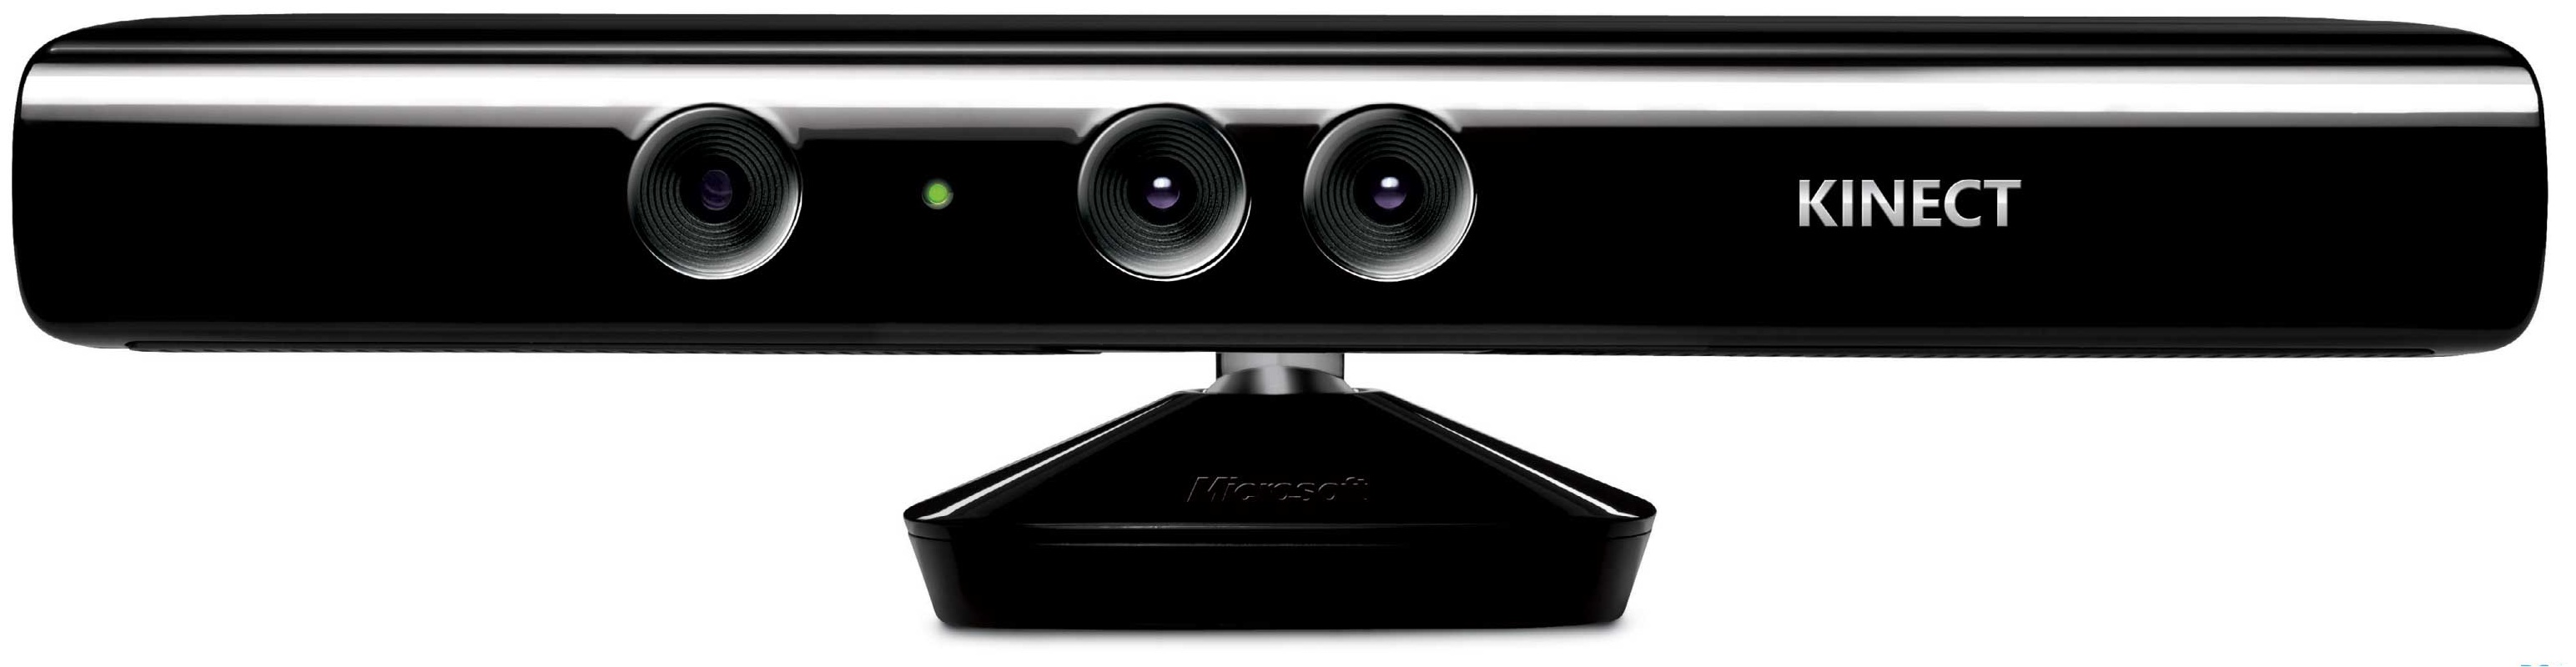
\includegraphics[scale=0.15]{./Figuras/KinectFrontal}
	\end{center}
	\caption{Vista frontal del Kinect}
	\label{fig:Kinect}
\end{figure}

Dentro del recubrimiento del sensor, un Kinect para Windows contiene:

\begin{itemize}
\item Una cámara RGB que almacena 3 canales de datos en una resolución de 1280x960. Esto permite capturar imágenes a color.
\item Un emisor infrarrojo (IR) y un sensor infrarrojo de profundidad. El emisor emite destellos de luz infrarroja y el sensor de profundidad lee los haces de luz infrarroja reflejadas de nuevo al sensor. Los haces reflejados son convertidos en información de profundidad midiendo la distancia entre un objeto y el sensor. Esto permite capturar la profundidad de una imagen.
\item Un micrófono multi-array, el cual contiene 4 micrófonos para capturar sonido. Debido a los 4 micrófonos, es posible grabar audio, así como encontrar la ubicación de la fuente de sonido y la dirección de la onda de audio.
\item Un acelerómetro de 3 ejes configurado para rango 2G donde la G es la aceleración debida a la gravedad. Es posible usar el acelerómetro para determinar la orientación actual del Kinect \cite{Microsoft3}.
\end{itemize}

\begin{figure}[h]%La h significa que la colocara cerca del texto
	\begin{center}
		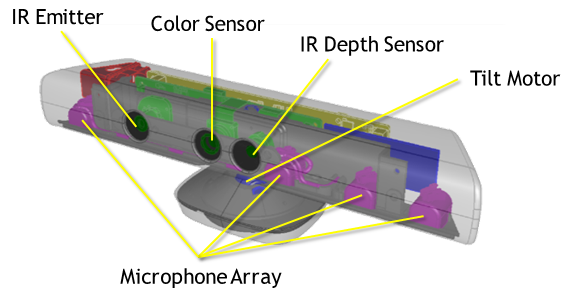
\includegraphics[scale=1]{./Figuras/KinectHardware}
	\end{center}
	\caption{Hardware interno del Kinect}
	\label{fig:KinectHardware}
\end{figure}
%------------------------------------------------------------------------------------
\subsection{Kinect SDK}
Microsoft Kinect SDK, provee las herramientas y API's necesarias para desarrollar aplicaciones para Microsoft Windows usando la tecnología de sensores de Kinect \cite{MicrosoftSDK}.\\

Existen 4 actualizaciones de la versión de SDK para el sensor Kinect, de las cuales la 1.8 es la versión a utilizar en el presente trabajo terminal, algunas características que se tienen hasta el momento son:
\begin{itemize}
\item Kinect Studio: Herramienta que permite a los desarrolladores grabar y reproducir datos de Kinect.
\item Reconocimiento del esqueleto ``sentado": Permite el seguimiento de 10 puntos (cabeza, cuello y brazos) ignorando las piernas y la cintura.
\item Datos ampliados profundidad: Las aplicaciones serán capaces de leer los datos más allá de cuatro metros cuando sea necesario.                                                                                                                  
\item APIs de configuración de la cámara a color: Los ajustes de la cámara de color se pueden optimizar para su entorno.
\item Nueva API de conversión de coordenadas espacio: Hay dos conjuntos de APIs, uno para la conversión de los píxeles individuales y la otra para la conversión de un cuadro de imagen completa.
\item Kinect Interactions: Ofrece la posibilidad a los desarrolladores de crear aplicaciones intuitivas que utilicen los gestos más comunes de la gente.
\item Kinect for Windows Interactions: Transforma la manera en la que la gente se comunica con la computadora.
\item Incluye herramientas de desarrollo mejoradas y más recursos para los desarrolladores tales como: Ejemplos de OpenCV y MATLAB compatibles con Kinect, ejemplos de código de Kinect para Windows para CodePlex ofreciendo la posibilidad de desarrollar en una plataforma open-source \cite{Heddle1}.
\end{itemize} 

Las características principales de la última versión (1.8) incluyen: 
\begin{itemize}
\item Un nuevo efecto de pantalla verde: Permite borrar el fondo detrás del usuario activo y después intercambiarlo por un fondo artificial.
\item Capacidades mejoradas para modelado en 3D: Permiten escanear el color de una escena al igual que sus contornos, lo que hace posible la impresión de objetos en 3D a todo color o pueda agregarse fidelidad a las características de los juegos y otras aplicaciones.
\item Una muestra de interfaz de usuario adaptable: Muestra cómo construir una aplicación que se adapta de acuerdo con la distancia entre el usuario y la pantalla para detección de gestos y tacto \cite{Heddle2}.
\end{itemize}
%------------------------------------------------------------------------------------
\subsection{Kinect SDK Open Source}
\subsubsection{OpenNI (Open Natural Interaction)}
Es un framework de código abierto creado por la empresa PrimeSense, permite comunicarse con los sensores de audio, video y sensor de profundidad de Kinect, mientras que proporciona una API que sirve de puente entre el hardware del equipo, NITE Middleware y las aplicaciones e interfaces del Sistema Operativo.  Su idea es facilitar el desarrollo de aplicaciones que funcionen con interacción natural, como gestos y movimientos corporales \cite{Echeverria}. \\

En noviembre del 2013, Apple compró la empresa PrimeSense. El 23 de abril del 2014, la página de OpenNI cerró y la descarga del software quedó deshabilitada desde esa fecha \cite{Armstrong}.

\subsubsection{OpenKinect}
Su objetivo principal actualmente es el software libfreenect, éste incluye todo el código necesario para activar, inicializar y comunicar los datos con el hardware de Kinect. La API  tiene enlaces y extensiones para los siguientes idiomas y plataformas: C, C++, NET (C\#), Java, Python, C y la interfaz síncrona.\\

OpenKinect también tiene como proyecto, la librería de análisis la cual se comunica con el API y analiza la información en bruto en abstracciones más útiles; así como aplicaciones, que incluyan códigos de ejemplo, demos, o cualquier aplicación que los usuarios quieran compartir.\\

El usuario que contribuya, puede optar por utilizar el proyecto con la licencia Apache 2.0 o licencia GPL v2 \cite{OpenKinect}. 
%------------------------------------------------------------------------------------
\section{Interfaz Natural de Usuario (INU)}

Existen diferentes definiciones de Interfaz natural de usuario tal como lo puntualizan los siguientes autores: \\

Una Interfaz natural de usuario es una interfaz de usuario diseñada para reutilizar habilidades existentes para interactuar directamente con contenido. ``Interfaz natural de usuario es la nueva forma de pensamiento acerca de como podemos interactuar con dispositivos de computación" \cite{Blake}. \\

La Interfaz natural de usuario (INU) es una evolución de la interfaz gráfica de usuario (GUI) y surge como un mecanismo de interacción hombre-máquina que permite establecer una  comunicación con sistemas computacionales a través de periféricos que pueden recibir instrucciones e información. La INU tiene algunas consideraciones adicionales las cuales se enfocan en hacer uso de una comunicación de manera natural con el ser humano, haciendo uso del captar información en tiempo real logrando una interacción corporal de manera directa, sin utilizar un periférico que actúe como intermediario para la entrada de información \cite{Gomez}. \\

La INU fundamenta sus principios en lo siguiente: debe ser directo, intuitivo e invisible al usuario (o hacerse invisible por medio de interacciones sencillas explicadas al usuario). No tiene que ser aprendido, porque está basado en elementos naturales, es decir, en los comandos utilizados en los comportamientos humanos habituales. Integra armoniosamente un balance entre fisiología y kinesiología, creando una interfaz para dedos vivos, no para cursores \cite{Sarajevo}. \\

\textbf{¿Qué significa natural?} \\

Una interfaz natural es aquella que ``explota las habilidades que hemos adquirido a través del tiempo vivido en el mundo" \cite{Buxton}. \\

La descripción anterior es interesante por dos razones. Primero, relaciona el concepto natural con la idea de rehusar habilidades existentes. Segundo, hace explícito que estas habilidades no son solamente habilidades innatas con las cuales nacimos. Natural significa usar habilidades innatas mas habilidades aprendidas y que hemos desarrollado a través de la interacción con nuestro propio ambiente natural cada día de la vida. \\

\textbf{¿Qué es una habilidad simple?} \\

Las habilidades simples solo dependen de las habilidades innatas aprendidas. Esto limita su complejidad, lo que también significa que son fáciles de aprender, tienen una baja carga cognitiva, y pueden ser rehusadas y adaptadas para muchos objetivo sin mucho esfuerzo. El proceso de aprendizaje de habilidades simples es típicamente muy veloz y requiere poca o ninguna práctica para alcanzar un adecuado nivel de competencia. En muchas ocasiones, este aprendizaje se puede alcanzar simplemente observando a alguien mas demonstrar la habilidad una o dos veces \cite{Blake}.

\subsection{Características de una Interfaz natural de usuario} 

\textbf{Centrada en el usuario} \\

Se toman como partida las necesidades cambiantes de la interfaz de usuario, de manera que se modifica la interfaz de usuario de la forma externa y los mecanismos internos para satisfacer las necesidades de los diferentes usuarios, lo cual es llamado diseño centrado en el usuario. La tecnología de reconocimiento de voz no específica de discursos humanos permitirá a las computadoras comprender las demandas de las personas, esta es una interfaz de entrada importante. \\

La tecnología fisheye observa la posición de los alrededores de un contenido con respecto a una posición en la pantalla, la cual es aumentada y es llamada observación amigable del usuario. En los sistemas tradicionales humano-maquina, las personas son consideradas como los operadores, es decir, personas que se adaptan a la máquina; en los sistemas generales hombre-máquina, las personas son conocidas como usuarios, pueden dialogar con la máquina, pero no tienen el control activo; en los sistemas de realidad virtual, las personas son participantes activos, donde la máquina responderá a diferentes acciones humanas. \\

\textbf{Multicanal} \\

Las interfaces multicanal tienen la intención de hacer un uso completo de uno o más de los canales sensores y motores, para capturar las características complementarias de los propósitos de los usuarios, para mejorar la naturalidad de la interacción hombre-máquina. \\

Los sentidos sensoriales humanos son la visión, el oído, el tacto, el olfato y el gusto; los canales de gestos humanos son las manos, la boca, los ojos, la cabeza, los pies, el cuerpo y así sucesivamente. Ahora, para las operaciones computacionales, los ojos humanos y las manos están muy cansados y la eficiencia no es alta \cite{Weiyuan}. Si escuchamos a, por ejemplo, la coordinación mano-ojo y otras acciones multicanal, se puede lograr una interacción natural y una comunicación humano-máquina eficiente así como brindar la posibilidad de elegir el mejor canal de respuesta posible, de tal manera que no se haga una sobrecarga sobre dichos canales. \\

\textbf{Inexacta} \\

La tecnología interactiva precisa, es una tecnología que puede ser usada para explicar completamente el propósito de las interacciones del usuario. El teclado y el ratón son necesarios para ingresar datos con precisión, pero las acciones de las personas o pensamientos no son muy precisos. Las computadores deben entender las peticiones de las personas e incluso corregir sus errores. Una interfaz que sea inteligente es una orientación importante. \\

\textbf{Alto ancho de banda} \\

Ahora las salidas de una computadora tienen que ser rápidas, con un continuo despliegue de imágenes a color y de una gran cantidad de información. Pero las personas aún utilizan como entrada el teclado en una que otra ocasión, por lo cual el ancho de banda es muy bajo. Las Interfaces naturales de usuario deben soportar un ancho de banda de entrada alto y una rápida importación de grandes cantidades de información. La entrada y entendimiento de voz, imagen, y la postura es una orientación de desarrollo para la actualidad y el futuro. \\

\textbf{Interacciones basadas en voz} \\

El lenguaje ha sido reconocido por mucho tiempo como el flujo más natural, conveniente y eficiente para el intercambio de información. En la vida diaria la comunicación humana es en un 75\% ejecutada por voz \cite{Weiyuan}. Los resultados muestran que existen muchas ventajas sobre los canales auditivos, como que la detección de canales auditivos es más rápida que la velocidad de detección de señales visuales. El cambio de un sonido personal es extremadamente sensible; la información auditiva y visual puede proporcionar el acceso a más personas hacia la existencia de un fuerte sentido de realismo, etc. Por lo tanto, el canal auditivo es el mas importante canal de interacción entre una computadora y otro dispositivo de información \cite{Weiyuan}. \\

La interacción por voz es una interacción con tecnología computacional para estudiar el como las personas interactúan a través de voz o voz sintetizadas por máquina. Esto involucra diferentes disciplinas como lingüística, psicología, ergonomía y tecnologías de la computación; al mismo tiempo es una visión hacía el futuro dirigido a la interacción por voz, su diseño y desarrollo. \\

Los sistemas interactivos por voz típicamente toman dos aproximaciones: una es basada en una tecnología de reconocimiento y entendimiento, que depende principalmente del sistema de audio con el que se interactúa; el otro es el uso de una tecnología de voz y de sistemas combinados en otras formas para interactuar con el sistema. De esta forma, la voz ya no es dominante sino sólo una parte de un sistema interactivo. \\

\textbf{Interacción basada en imagen} \\

La interacción por imagen simplemente es una computadora basada en comportamiento humano que entiende una imagen y entonces reacciona. \\

En el presente, los sistemas de visión artificial se pueden dividir en 3 niveles: el procesamiento de imagen (al más bajo nivel), el reconocimiento de imágenes (a un alto nivel) y la percepción de imágenes (al más alto nivel). El procesamiento de imágenes es el proceso de ingresar una imagen como entrada y de tener una imagen a la salida \cite{Weiyuan}. El reconocimiento de patrones, se interesa principalmente en la detección de objetivos en la imagen y su medición, para obtener información objetiva, con el fin de establecer la descripción de la imagen. Esencialmente es el proceso de llevar una imagen a datos. \\

La percepción de imagen se centra en estudiar aún más la naturaleza de la imagen de destino y sus relaciones mutuas sobre la base del reconocimiento de imágenes, y viene para entender el significado del contenido de una imagen e interpretación de la escena original. En la percepción de imágenes, la entrada es una imagen y la salida es una interpretación de dicha imagen. \\

\textbf{Interacciones basadas en comportamiento} \\

En el proceso de intercambio, en adición a la interacción por voz, las personas frecuentemente utilizan el lenguaje corporal, el cual involucra movimientos del cuerpo para expresar su actitud y significado, por lo tanto, es un proceso basado en interacciones humanas. El método de interacciones por acciones humanas puede no solamente mejorar las habilidades de lenguajes, sino también, puede jugar el rol de interacción que la voz no puede. \\

El comportamiento de la interacción humano-computadora es el reconocimiento de comportamiento humano a través de posicionamiento, seguimiento, movimiento y expresión de las partes del cuerpo para entender las acciones y el comportamiento, y responder con un proceso inteligente de retroalimentación. \\

Las interacciones basadas en comportamiento brindan una nueva forma de interacción. El comportamiento del usuario puede ser predecido por la computadora y así conocer las necesidades de los usuarios. Por ejemplo: con un seguimiento de la atención de las personas, se puede determinar la intención de los usuarios para visitar un sitio web especifico o la necesidad de una llamada; cuando el usuario entra en una habitación, la computadora responde enviándole un correo electrónico, si el usuario niega con la cabeza, el equipo considera que el usuario no desea leer el mensaje.
%------------------------------------------------------------------------------------
\section{Karate Do}
\label{sec:Karate-Do}
El Karate Do, en todas sus diferentes formas, encuentra sus orígenes en un sólo lugar, las islas Ryukyu fuera de la costa de Japón. Lo que se sabe de uno de los sistemas de entrenamiento de auto defensa y disciplina más practicados en el mundo es el resultado de siglos de desarrollo. \\

El Karate Do es un arte marcial tradicional en el que se coordina la fuerza, la respiración, el equilibrio y la postura, el correcto giro de cadera y la conexión conjunta de músculos y extremidades, trasladando gran parte del peso corporal y del centro de gravedad al impacto. Se caracteriza por el empleo de golpes de puño y patadas, aunque no restringe su repertorio sólo a ellos. Normalmente, un entrenamiento de Karate Do se divide en 5 partes que son: el calentamiento, los ejercicios de resistencia, la técnica, las Katas y el Kumite (o combate); el presente trabajo está enfocado en el aprendizaje de la técnica del Karate Do, por lo que se verán contemplados los ejercicios de calentamiento y los movimientos de técnica. \\

En la actualidad existen diferentes estilos en la enseñanza del Karate Do, todos basados en la técnica original, pero normalmente cambiando los métodos de enseñanza dependiendo de las regiones o incluso de cada instructor. Para el caso del presente trabajo terminal, se tiene el apoyo y asesoría del experto Moisés Gachúz Mendoza cuyo grado es de Cinta Negra 5to Dan registrado en la Federación Mexicana de Karate Do desde el 2005.
%------------------------------------------------------------------------------------
\subsection{Calentamiento}
\label{sec:Calentamiento}
El calentamiento es un aspecto importante para cualquier rutina de ejercicios. Realizar ejercicios de calentamiento antes de estiramientos, calienta la temperatura del cuerpo, lo cual incrementa el flujo de sangre en los músculos y los hace más flexibles. El calentamiento también protege al corazón, ya que las personas que calientan por al menos dos minutos antes de una rutina de ejercicios reducen su riesgo de alta presión sanguínea e incrementa el flujo de oxígeno en el corazón. El calentamiento debe ser la primera actividad realizada antes de hacer estiramientos, ejercicio cardiovascular o entrenamiento de resistencia \cite{Nall}.\\

Existen ejercicios de calentamiento recomendados especialmente para cada tipo de actividad física o deportiva, el Karate Do es un deporte que no se enfoca en una sola actividad, sino que tiene una combinación de varias, como los ejercicios de resistencia, el estiramiento o los ejercicios cardiovasculares; es por ello que para el presente trabajo terminal se proponen rutinas de entrenamiento con los siguientes ejercicios de calentamiento, Figura \ref{fig:Musculos_Cuello} - Figura \ref{fig:Musculos_Estiramiento3}, indicados como parte del Programa Nacional de Activación Física de la CONADE \cite{CONADE}:

\clearpage

\begin{figure}[H]
	\centering
	\subfloat[Flexión lateral del cuello, izquierdo y derecho]{
		\label{fig:Cuello_Frontal}
		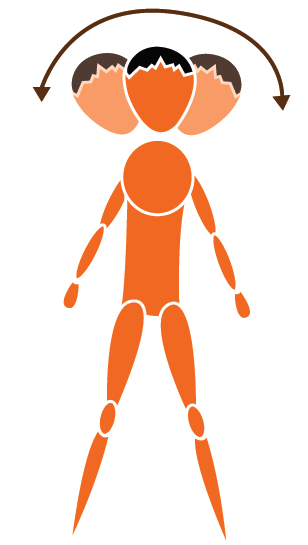
\includegraphics[width=4.5cm, height=8cm]{./Figuras/Calentamiento/1_Flexion_lateral_del_cuello}}
	\subfloat[Flexión del cuello al frente y extensión del cuello atrás]{
		\label{fig:Cuello_Lateral}
		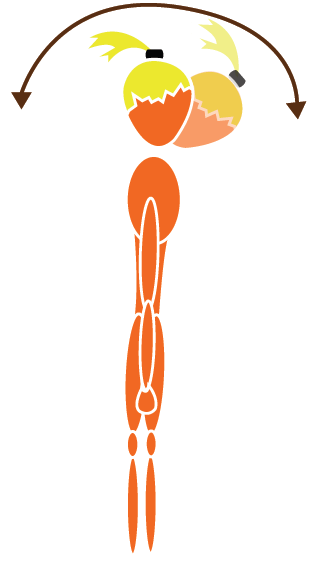
\includegraphics[width=5.5cm, height=8cm]{./Figuras/Calentamiento/2_Flexion_del_cuello_al_frente}}
	\caption{Músculos de cuello}
	\label{fig:Musculos_Cuello}
\end{figure}

\begin{figure}[H]
	\begin{center}
		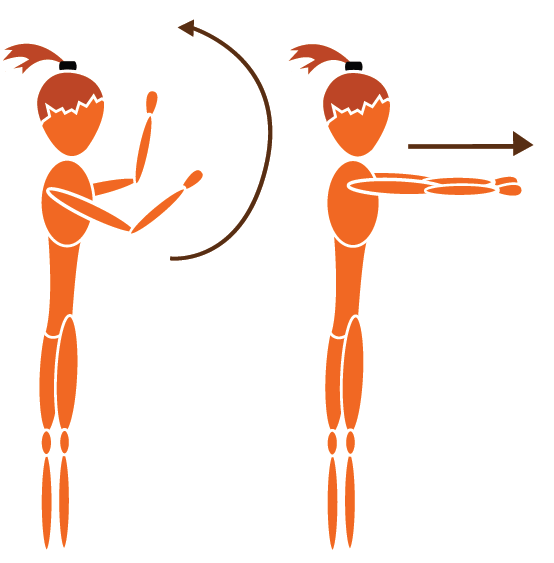
\includegraphics[width=8cm, height=8cm]{./Figuras/Calentamiento/7_Flexion_del_codo}\\
		Flexión y extensión del codo
	\end{center}
	\caption{Músculos del brazo}
	\label{fig:Musculos_Brazo}
\end{figure}

\begin{figure}[H]
	\centering
	\subfloat[Flexión y extensión del tronco(enfrente y atrás)]{
		\label{fig:Tronco_Frontal}
		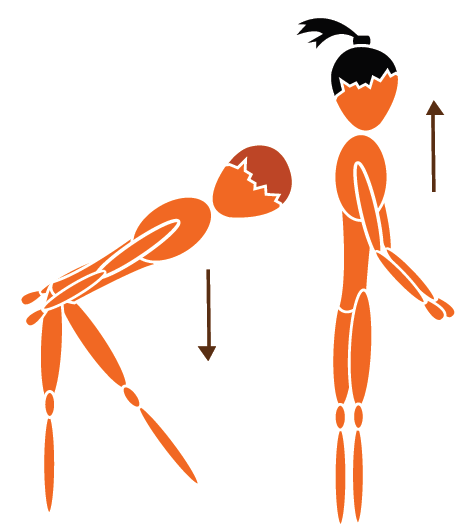
\includegraphics[width=7cm, height=8cm]{./Figuras/Calentamiento/12_Flexion_del_tronco}}
	\subfloat[Flexión del tronco izquierdo y derecho]{
		\label{fig:Tronco_Lateral}
		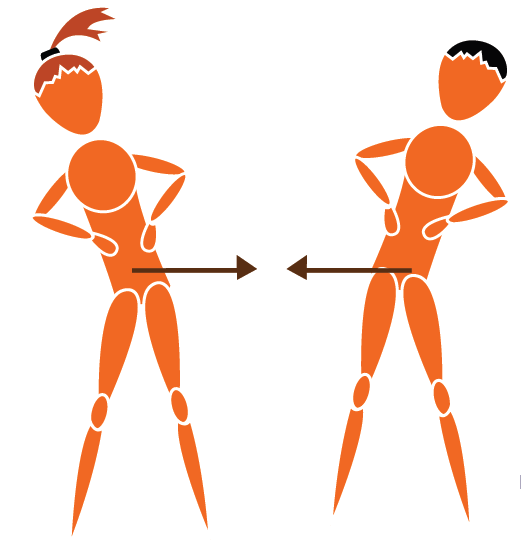
\includegraphics[width=5.5cm, height=8cm]{./Figuras/Calentamiento/13_Flexion_lateral_del_tronco}}
	\caption{Músculos de la cadera}
	\label{fig:Musculos_Cadera}
\end{figure}

\begin{figure}[H]
	\centering
	\subfloat[Flexión y extensión de rodilla]{
		\label{fig:Piernas_Frontal}
		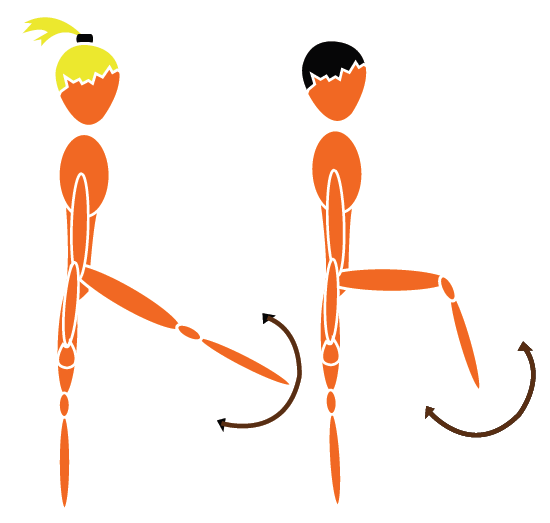
\includegraphics[width=8cm, height=8cm]{./Figuras/Calentamiento/15_Flexion_de_la_rodilla}}
	\subfloat[Abrir y cerrar las piernas derecha e izquierda]{
		\label{fig:Piernas_Lateral}
		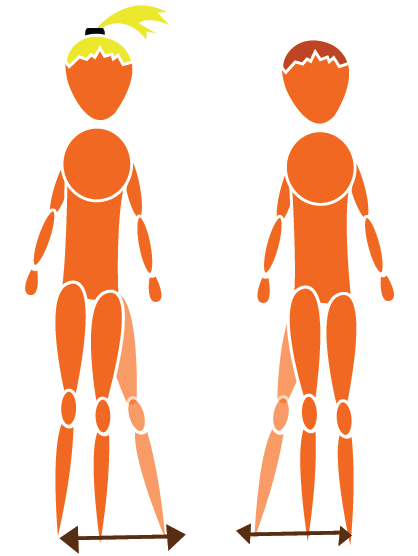
\includegraphics[width=5.5cm, height=8cm]{./Figuras/Calentamiento/16_Abrir_piernas}}
	\caption{Músculos de la pierna}
	\label{fig:Musculos_Pierna}
\end{figure}

\begin{figure}[H]
	\centering
	\subfloat[Estiramiento de músculos posteriores de la pierna]{
		\label{fig:Musculos_Estiramiento1}
		
\includegraphics[width=5.5cm, height=8cm]{./Figuras/Calentamiento/28_Estiramiento_de_musculos_de_la_pierna}}
	\subfloat[Estiramiento del músculo de la pierna]{
		\label{fig:Musculos_Estiramiento2}
		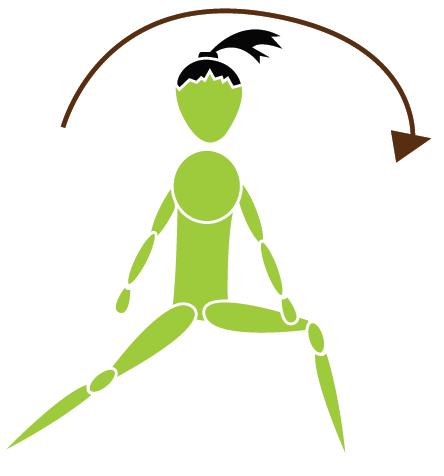
\includegraphics[width=5.5cm, height=8cm]{./Figuras/Calentamiento/29_Estiramiento_del_musculo_de_la_pierna}}
	\caption{Estiramientos de pierna}
	\label{fig:Estiramientos_Pierna}
\end{figure}

\begin{figure}[H]
	\begin{center}
		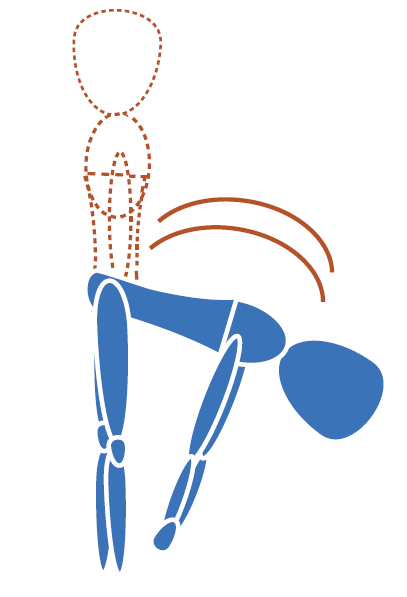
\includegraphics[width=5.5cm, height=8cm]{./Figuras/Calentamiento/44_lab_Flexion_de_tronco_al_frente}\\
		Separación de las piernas a la altura de los hombros, se flexiona el tronco tocando la punta de los pies
	\end{center}
	\caption{Estiramiento}
	\label{fig:Musculos_Estiramiento3}
\end{figure}

%-----------------------------------------------------------------------------
\subsubsection{Descripción de ejercicios}
La siguiente tabla muestra la lista de los ejercicios de calentamiento propuestos en la herramienta, describiendo la manera de realizarse y su utilidad en la realización de la técnica del Karate Do.

\begin{table}[H]
\centering
\begin{tabular}{| p{3 cm} | p{4 cm} | p{4 cm} | p{4 cm} |}
\hline
\rowcolor[rgb]{0.529412, 0.807843, 0.980392} {\textbf{Parte del cuerpo}} & {\textbf{Postura}} & {\textbf{Descripción}} & {\textbf{Técnica de Karate Do}}\\
\hline
\textbf{Calentamiento de músculos del cuello} &  Brazos extendidos a los costados.
Piernas ligeramente abiertas a la altura de los hombros. & Flexión lateral del cuello, hacia la izquierda y hacia la derecha. & Es necesario para realizar posiciones de manera precisa.\\
\hline
\textbf{Calentamiento de músculos del cuello} & Brazos extendidos a los costados.
Piernas ligeramente abiertas a la altura de los hombros. & Flexión del cuello hacia el frente y extensión del cuello hacia atrás. & Es necesario para realizar posiciones de manera precisa.\\
\hline
\textbf{Calentamiento de músculos del brazo} & Piernas ligeramente abiertas a la altura de los hombros.
Brazos levantados a la altura de los hombros. & Flexión y extensión de los codos. & Es necesario para realizar posiciones, ataques con brazo y defensas de manera precisa.\\
\hline
\textbf{Calentamiento de músculos de cadera} & Piernas separadas, superando la posición de los hombros. & Flexión y extensión del tronco, hacia enfrente y atrás. & Es necesario para realizar posiciones y ataques con pierna de manera precisa.\\		
\hline
\textbf{Calentamiento de músculos de cadera} & Piernas separadas, superando la posición de los hombros. & Flexión del tronco hacia los lados derecho e izquierdo. & Es necesario para realizar posiciones y ataques con pierna de manera precisa.\\
\hline
\textbf{Calentamiento de músculos de la pierna} & Una pierna en el suelo y la otra pierna levantada a la altura de la cadera. & Flexión y extensión de la rodilla de la pierna levantada. & Es necesario para realizar posiciones y ataques con pierna de manera precisa.\\
\hline
\textbf{Calentamiento de músculos de la pierna} & Piernas ligeramente abiertas a la altura de los hombros. & Abrir y cerrar las piernas (una a la vez) haciendo movimientos de derecha a izquierda.& Es necesario para realizar posiciones y ataques con pierna de manera precisa.\\
\hline


\end{tabular}
%\caption{Descripción de ejercicios de calentamiento}
\label{tab:DEC}
\end{table} 

\begin{table}[H]
\centering
\begin{tabular}{| p{3 cm} | p{4 cm} | p{4 cm} | p{4 cm} |}
\hline
\textbf{Estiramiento de músculos de la pierna} & Una pierna flexionada hacia el frente y la otra estirada hacia atrás. & Mantener la posición por unos segundos. & Es necesario para realizar posiciones de manera precisa, así como ataques con pierna con mayor fuerza y alcance.\\
\hline	
\textbf{Estiramiento de músculos de la pierna} & Con el cuerpo de frente se estira una pierna y la otra se flexiona. & Mantener la posición por unos segundos, recargando la mayor parte del peso sobre la pierna flexionada. & Es necesario para realizar posiciones de manera precisa, así como ataques con pierna con mayor fuerza y alcance.\\
\hline
\textbf{Estiramiento de piernas y cadera} & Piernas ligeramente separadas a la altura de los hombros. & Flexionar el tronco hacia enfrente, tocando la punta de los pies con las manos.
Mantener la posición por unos segundos. & Es necesario para realizar posiciones de manera precisa, así como ataques con pierna con mayor fuerza y alcance.\\
\hline
\end{tabular}
\caption{Descripción de ejercicios de calentamiento}
\label{tab:DEC2}
\end{table} 

%------------------------------------------------------------------------------------
\subsection{Técnica}
La técnica es un procedimiento o conjunto de reglas, normas o protocolos que tienen como objetivo obtener un resultado determinado.
Para el caso del Karate Do, la técnica hace referencia al conjunto de movimientos propios de dicho deporte, como son los ataques, las defensas, las posiciones , Katas y Kumite (combate); el presente trabajo terminal está enfocado en la técnica inicial de cinta blanca la cual contempla los primeros tres, tomando como referencia los movimientos específicos que se muestran a continuación, de la Figura \ref{fig:Posiciones1} a la Figura \ref{fig:Ataques2}:

\begin{figure}[H]
	\centering
	\subfloat[Musubi - dachi frontal]{
		\label{fig:Musubidachi_Frontal}
		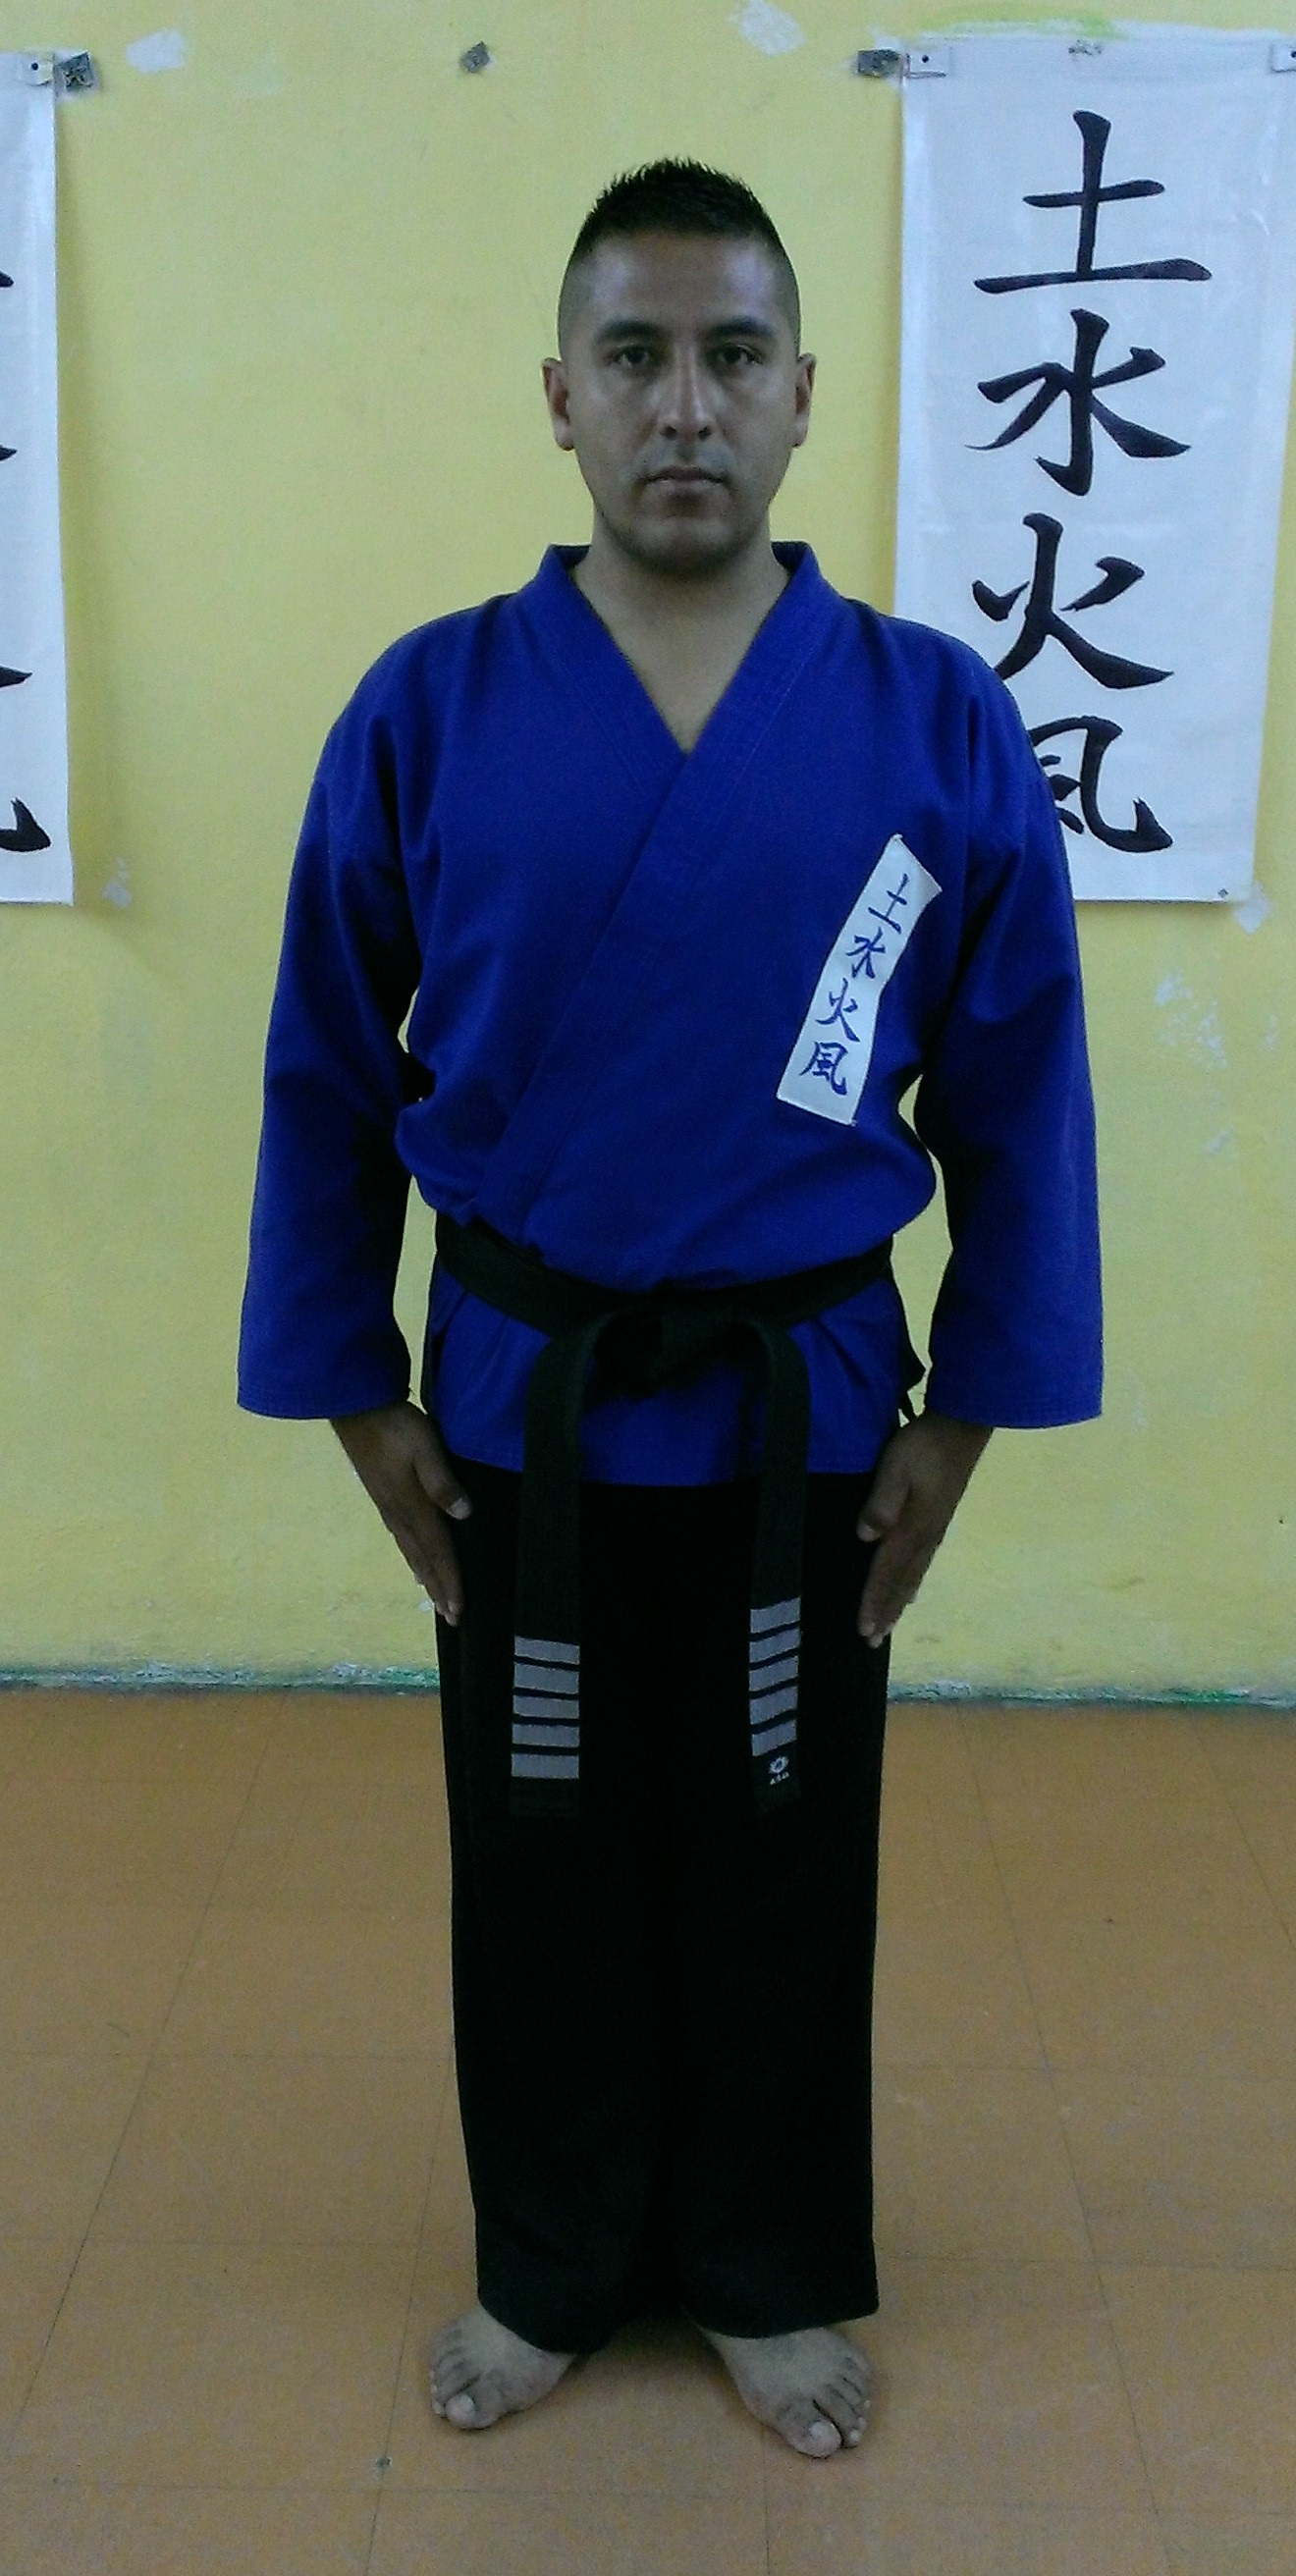
\includegraphics[width=4.5cm, height=8cm]{./Figuras/Tecnica/Musubidachi_Frontal}}
	\subfloat[Hachiji - dachi frontal]{
		\label{fig:Hachijidachi_Frontal}
		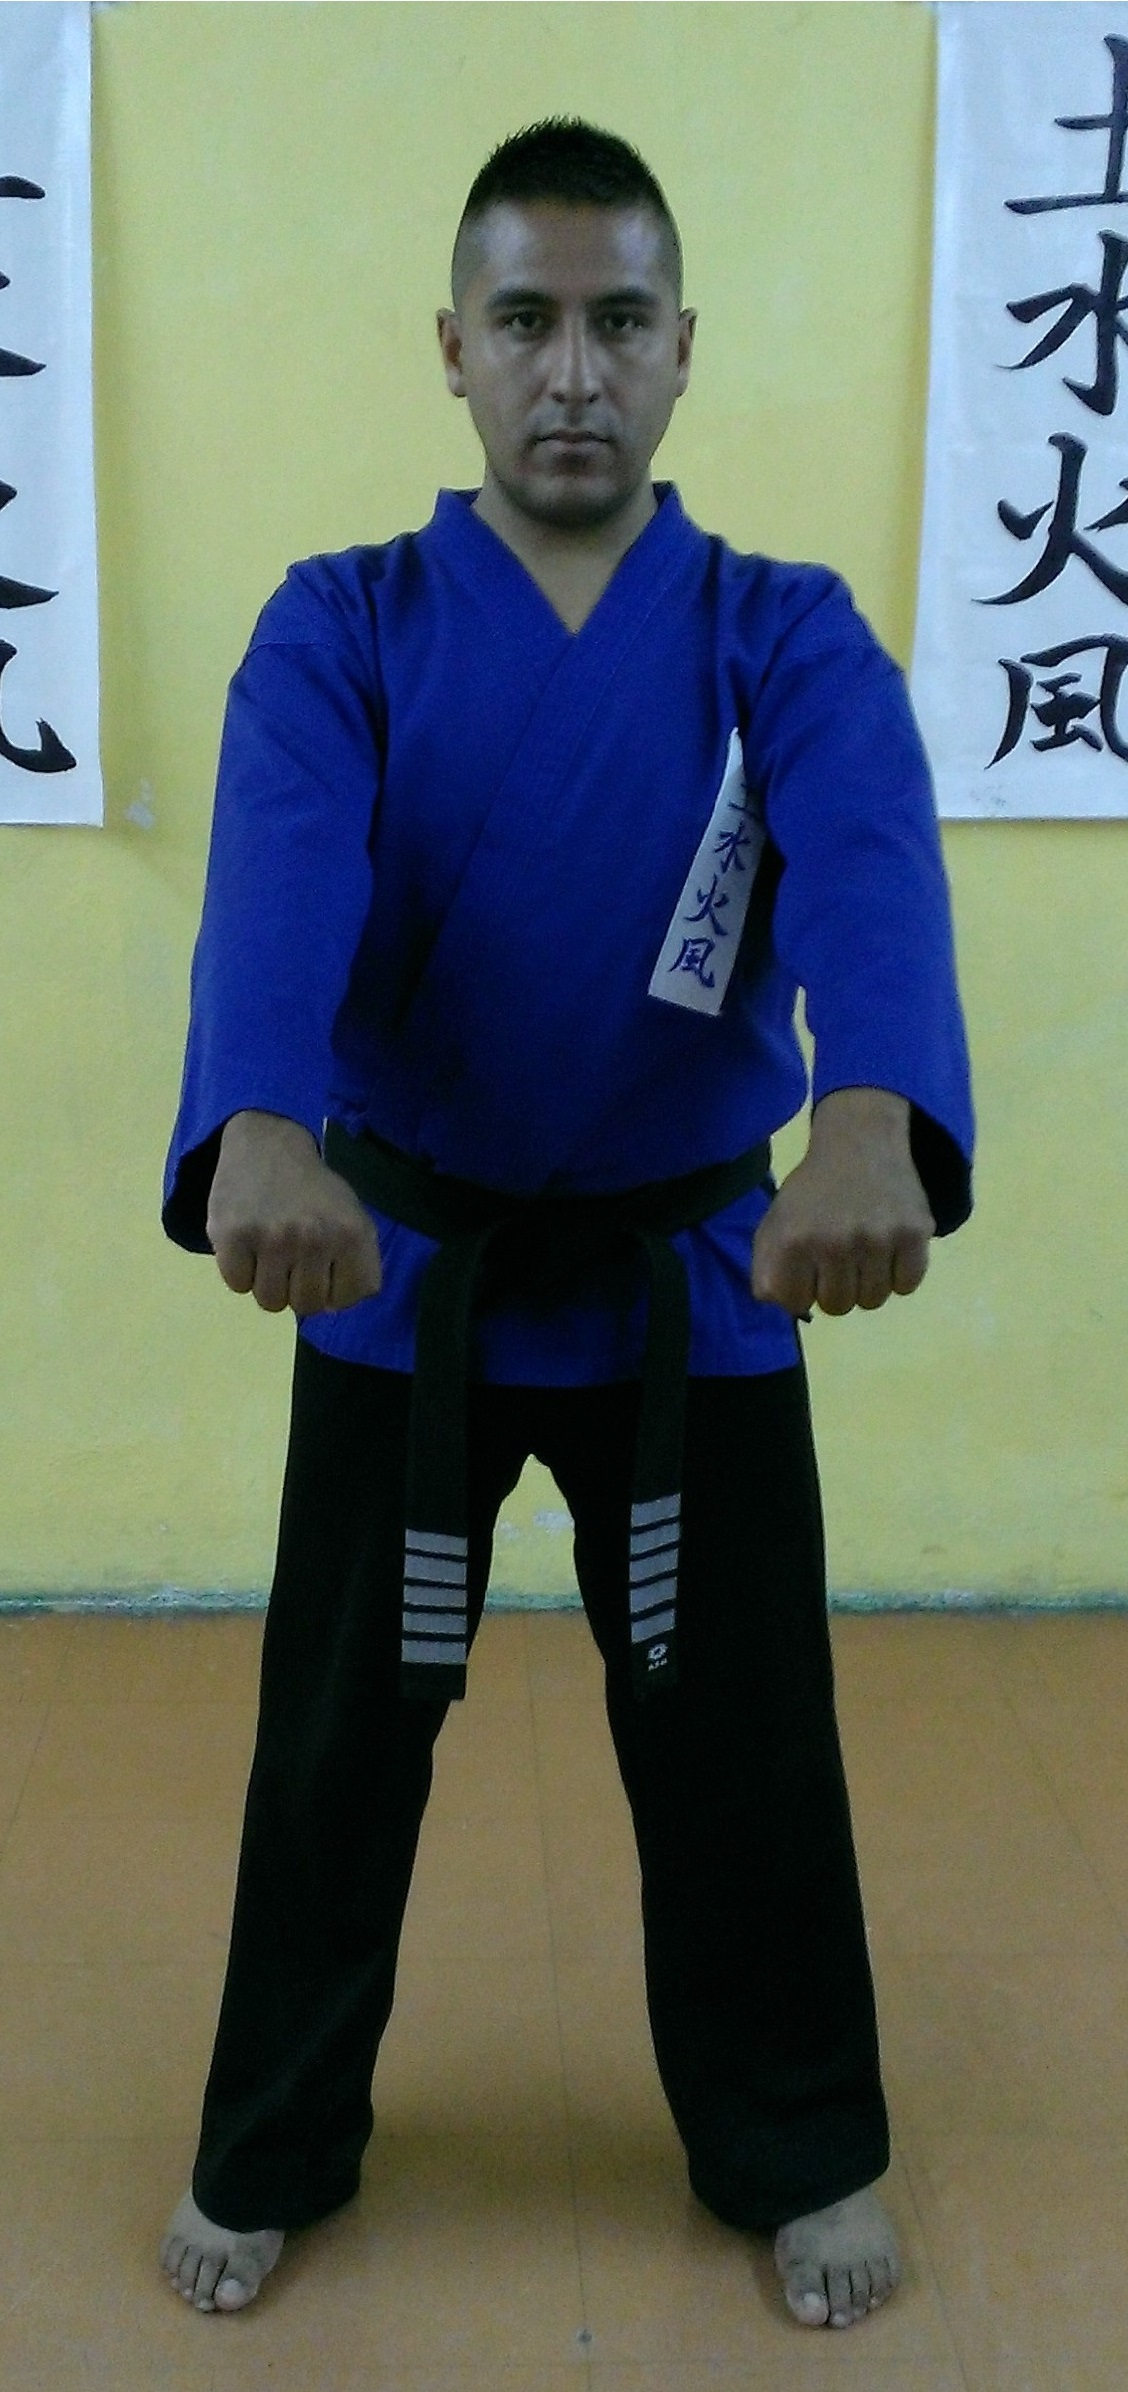
\includegraphics[width=4.5cm, height=8cm]{./Figuras/Tecnica/Hachijidachi_Frontal}}
	\caption{Posiciones Musubi - dachi y Hachiji - dachi }
	\label{fig:Posiciones1}
\end{figure}

\begin{figure}[H]
	\centering
	\subfloat[Posición Senkuntsu - dachi frontal]{
		\label{fig:Senkuntsudachi_Frontal}
		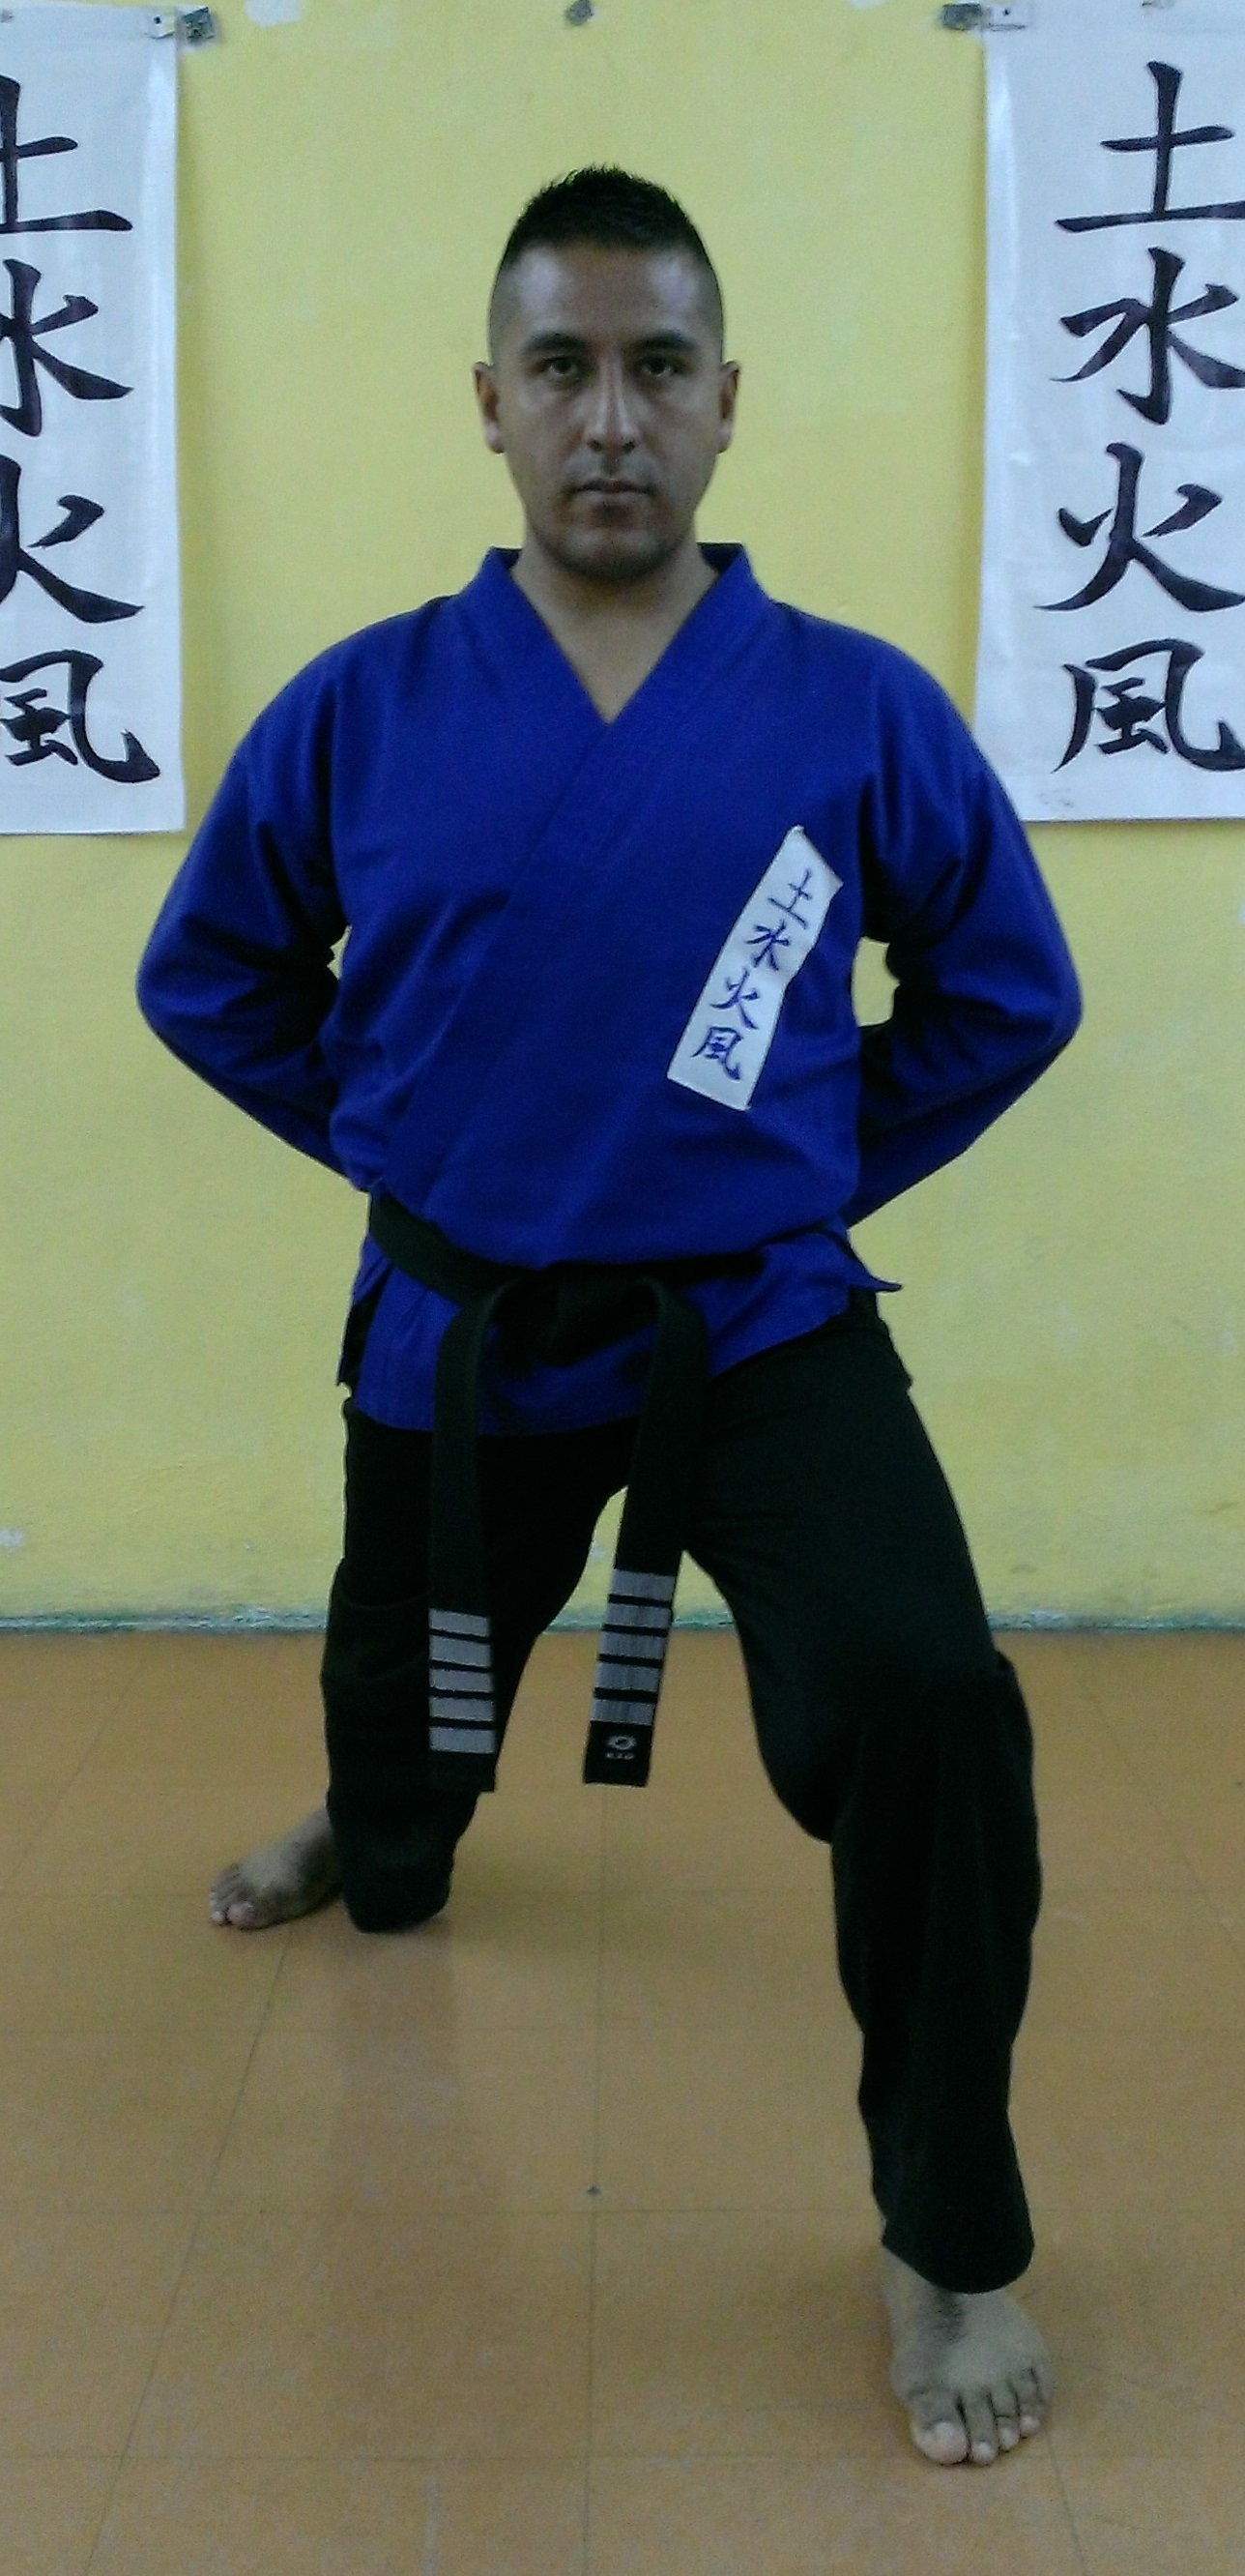
\includegraphics[width=4.5cm, height=8cm]{./Figuras/Tecnica/Senkuntsudachi_Frontal}}
	\subfloat[Posición Senkuntsu - dachi lateral]{
		\label{fig:Senkuntsudachi_Lateral}
		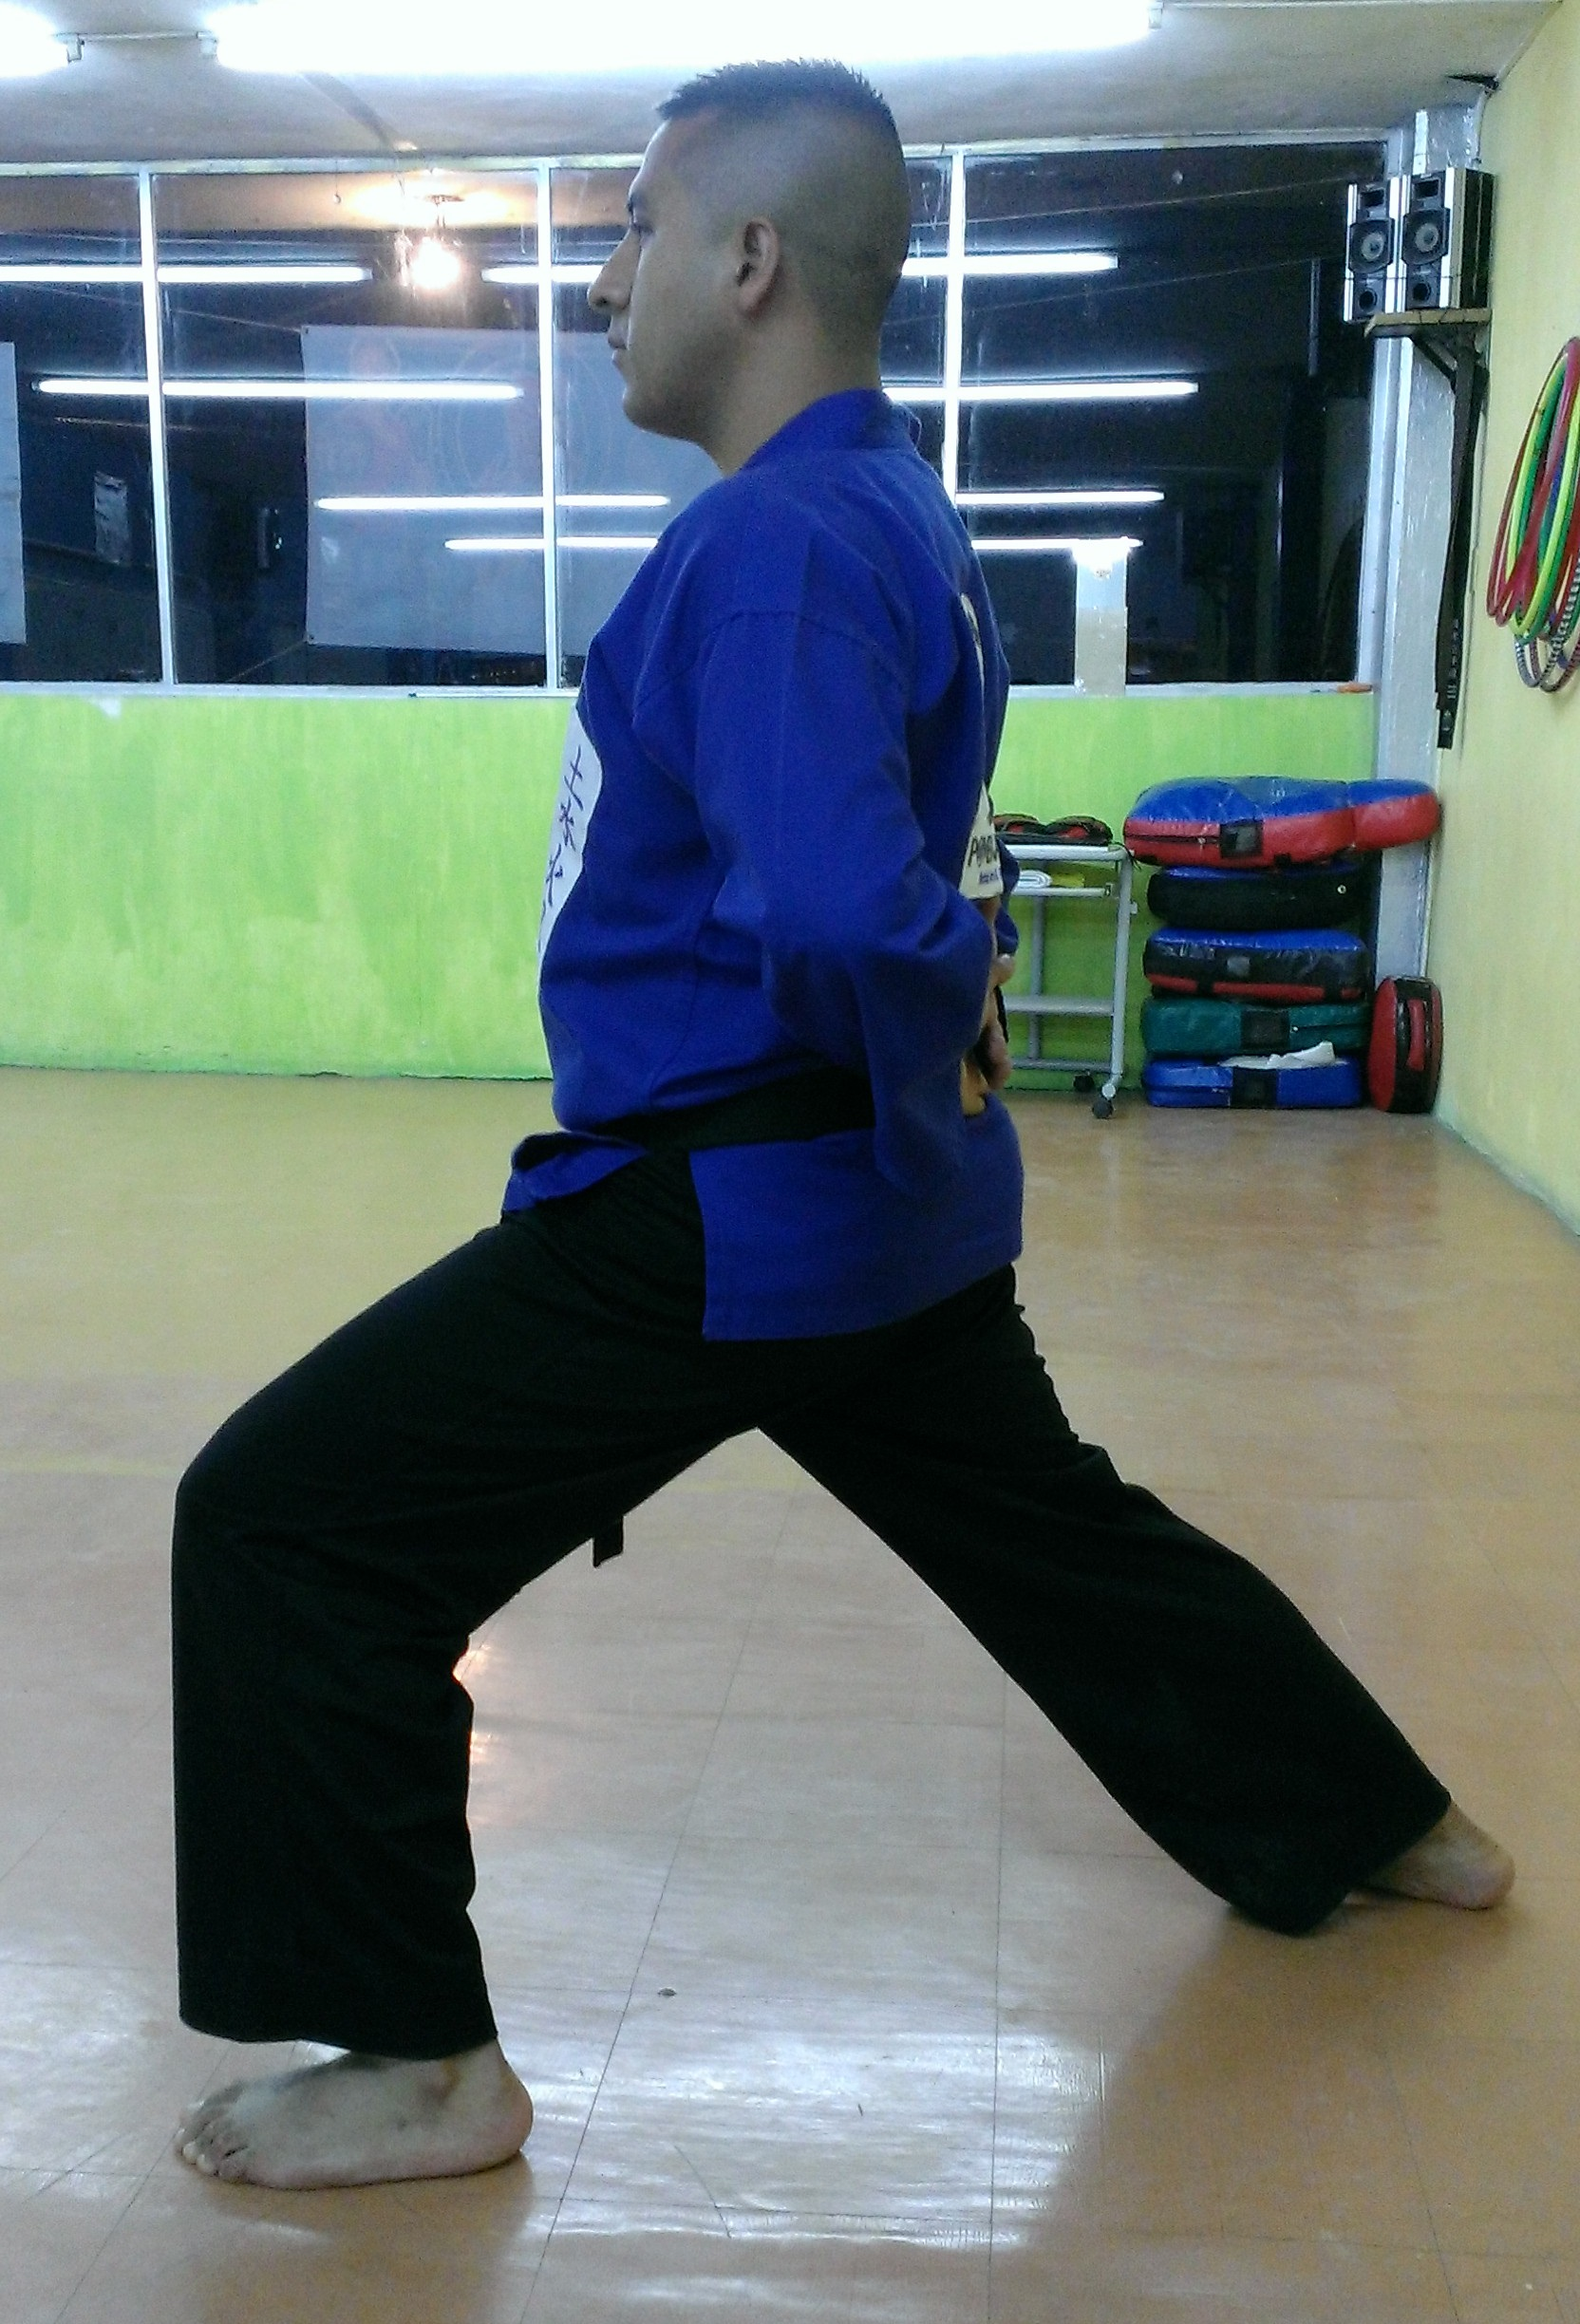
\includegraphics[width=5.5cm, height=8cm]{./Figuras/Tecnica/Senkuntsudachi_Lateral}}
	\caption{Posición Senkuntsu - dachi}
	\label{fig:Posiciones2}
\end{figure}

\begin{figure}[H]
	\centering
	\subfloat[Defensa Gedan Barai Uke frontal]{
		\label{fig:GedanBaraiUke_Frontal}
		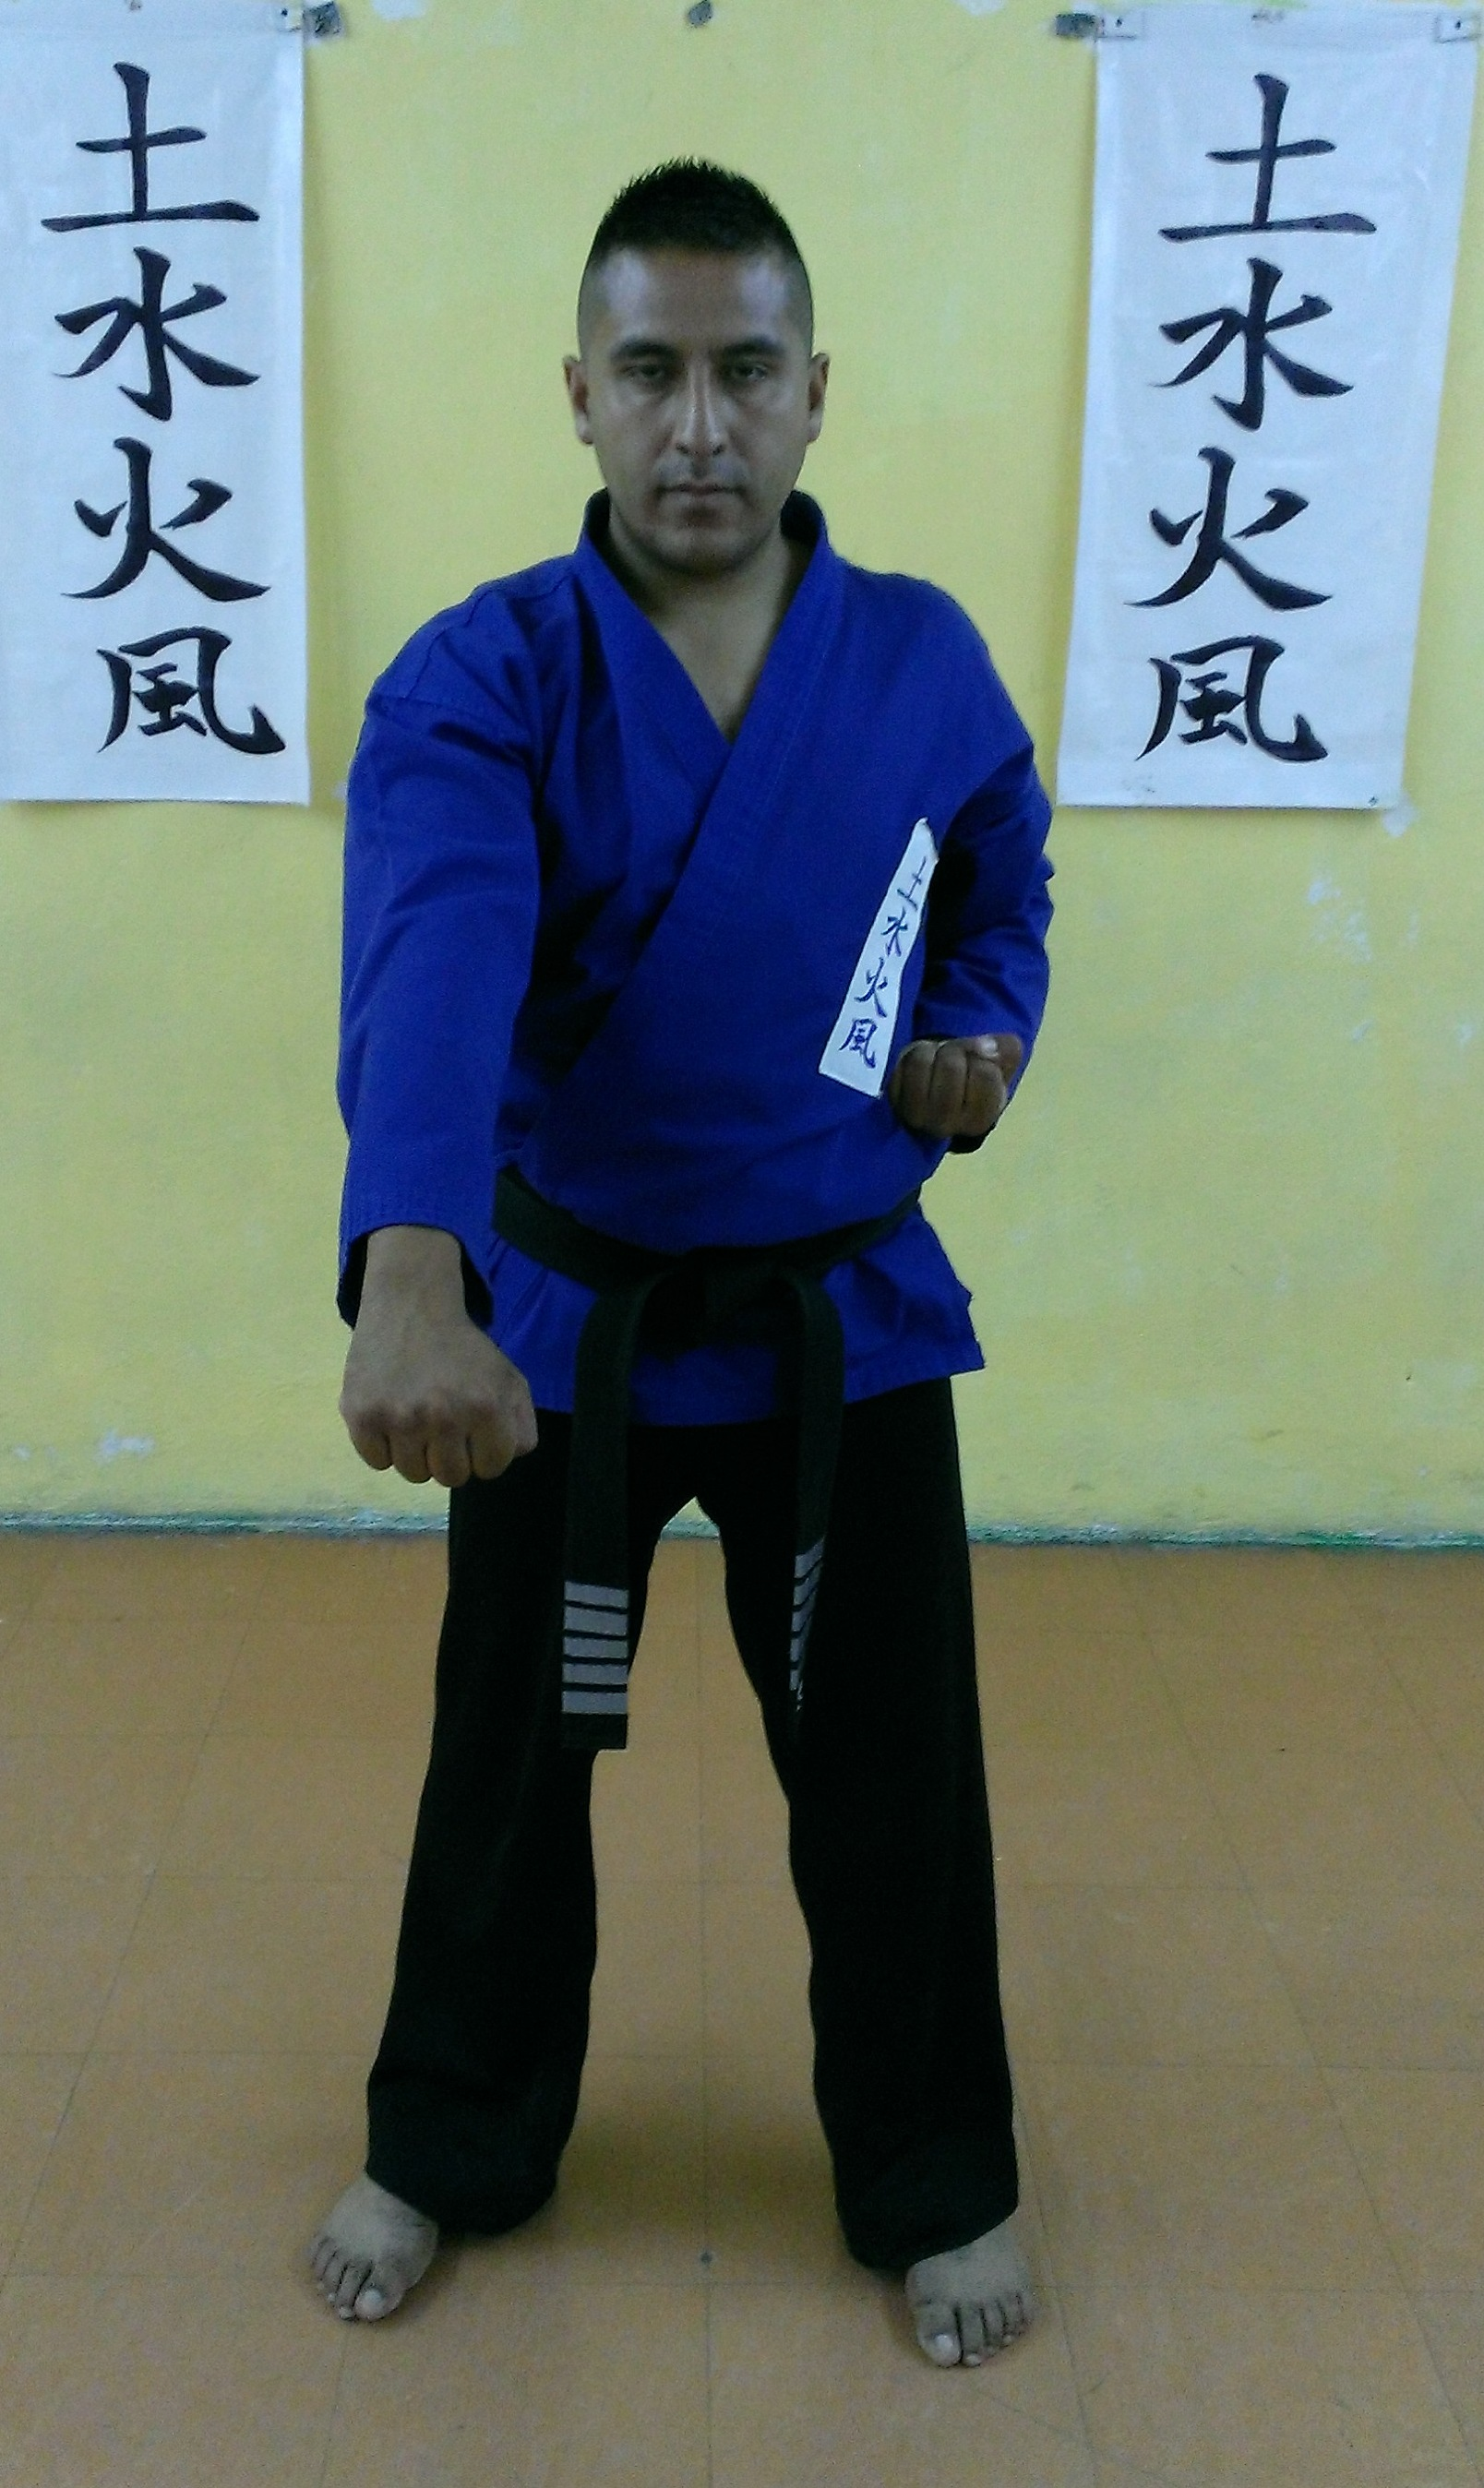
\includegraphics[width=5cm, height=8cm]{./Figuras/Tecnica/GedanBaraiUke_Frontal}}
	\subfloat[Defensa Gedan Barai Uke lateral]{
		\label{fig:GedanBaraiUke_Lateral}
		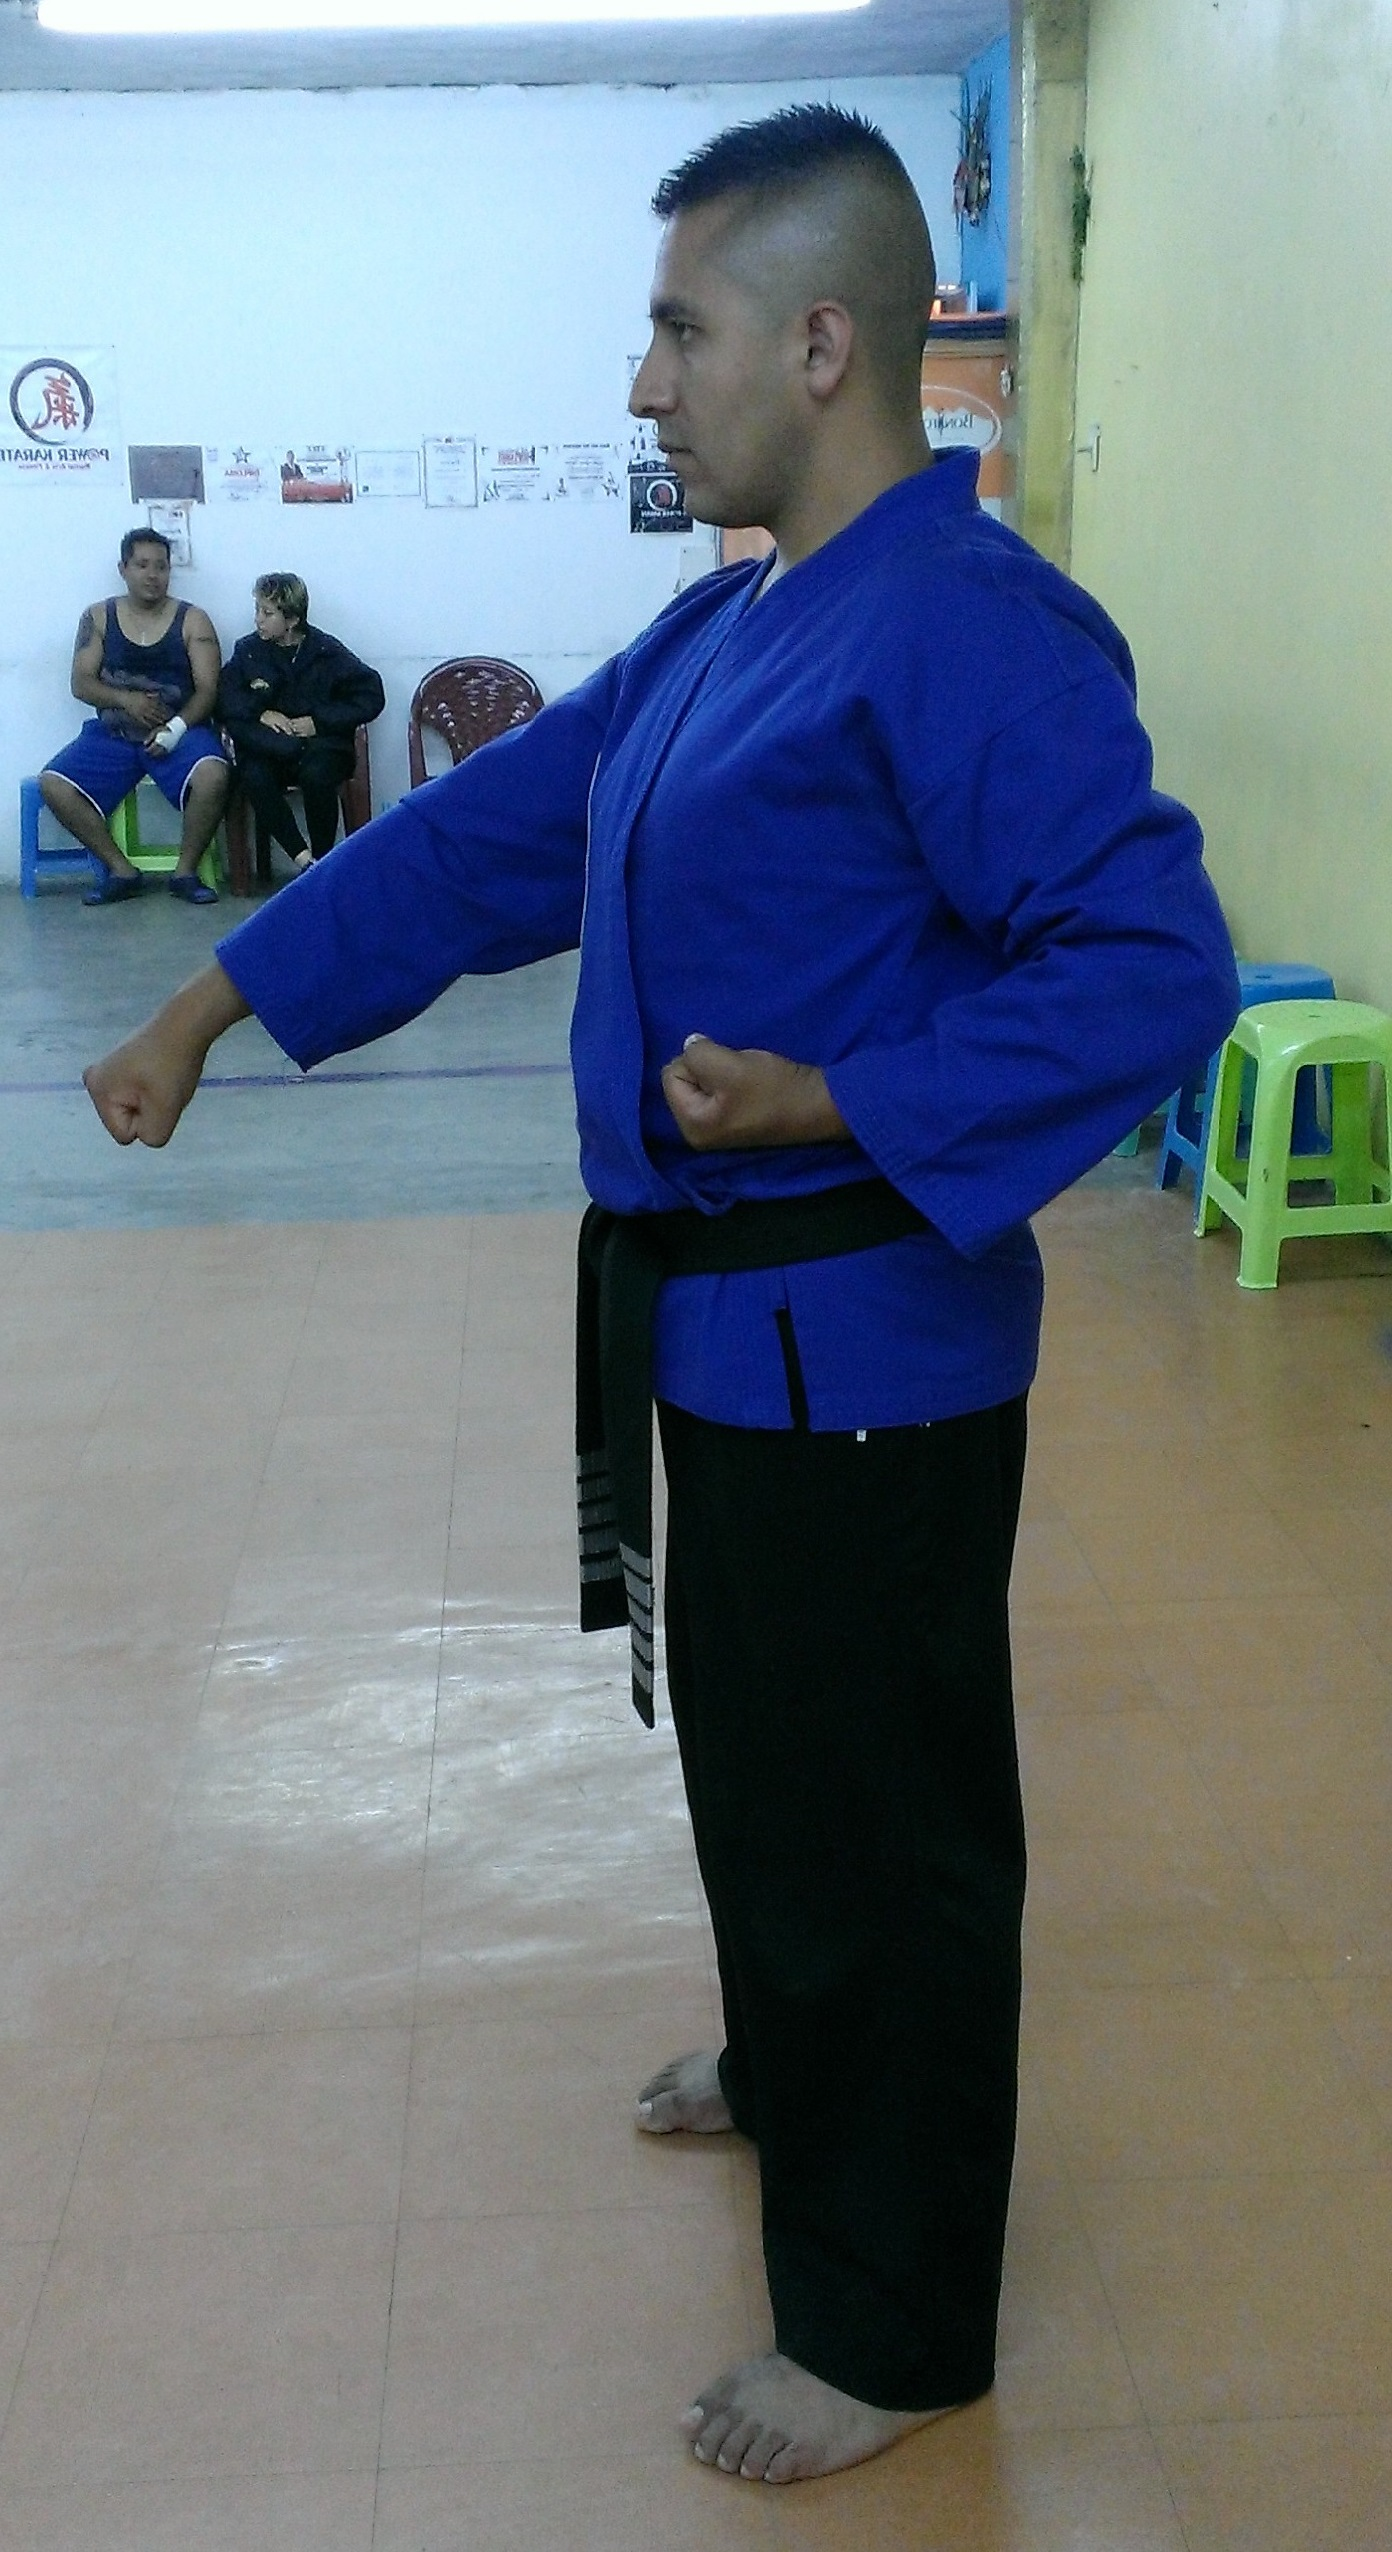
\includegraphics[width=5cm, height=8cm]{./Figuras/Tecnica/GedanBaraiUke_Lateral}}
	\caption{Defensa Gedan Barai Uke}
	\label{fig:Defensas1}
\end{figure}

\begin{figure}[H]
	\centering
	\subfloat[Defensa Shudan Soto Uke frontal]{
		\label{fig:ShudanSotoUke_Frontal}
		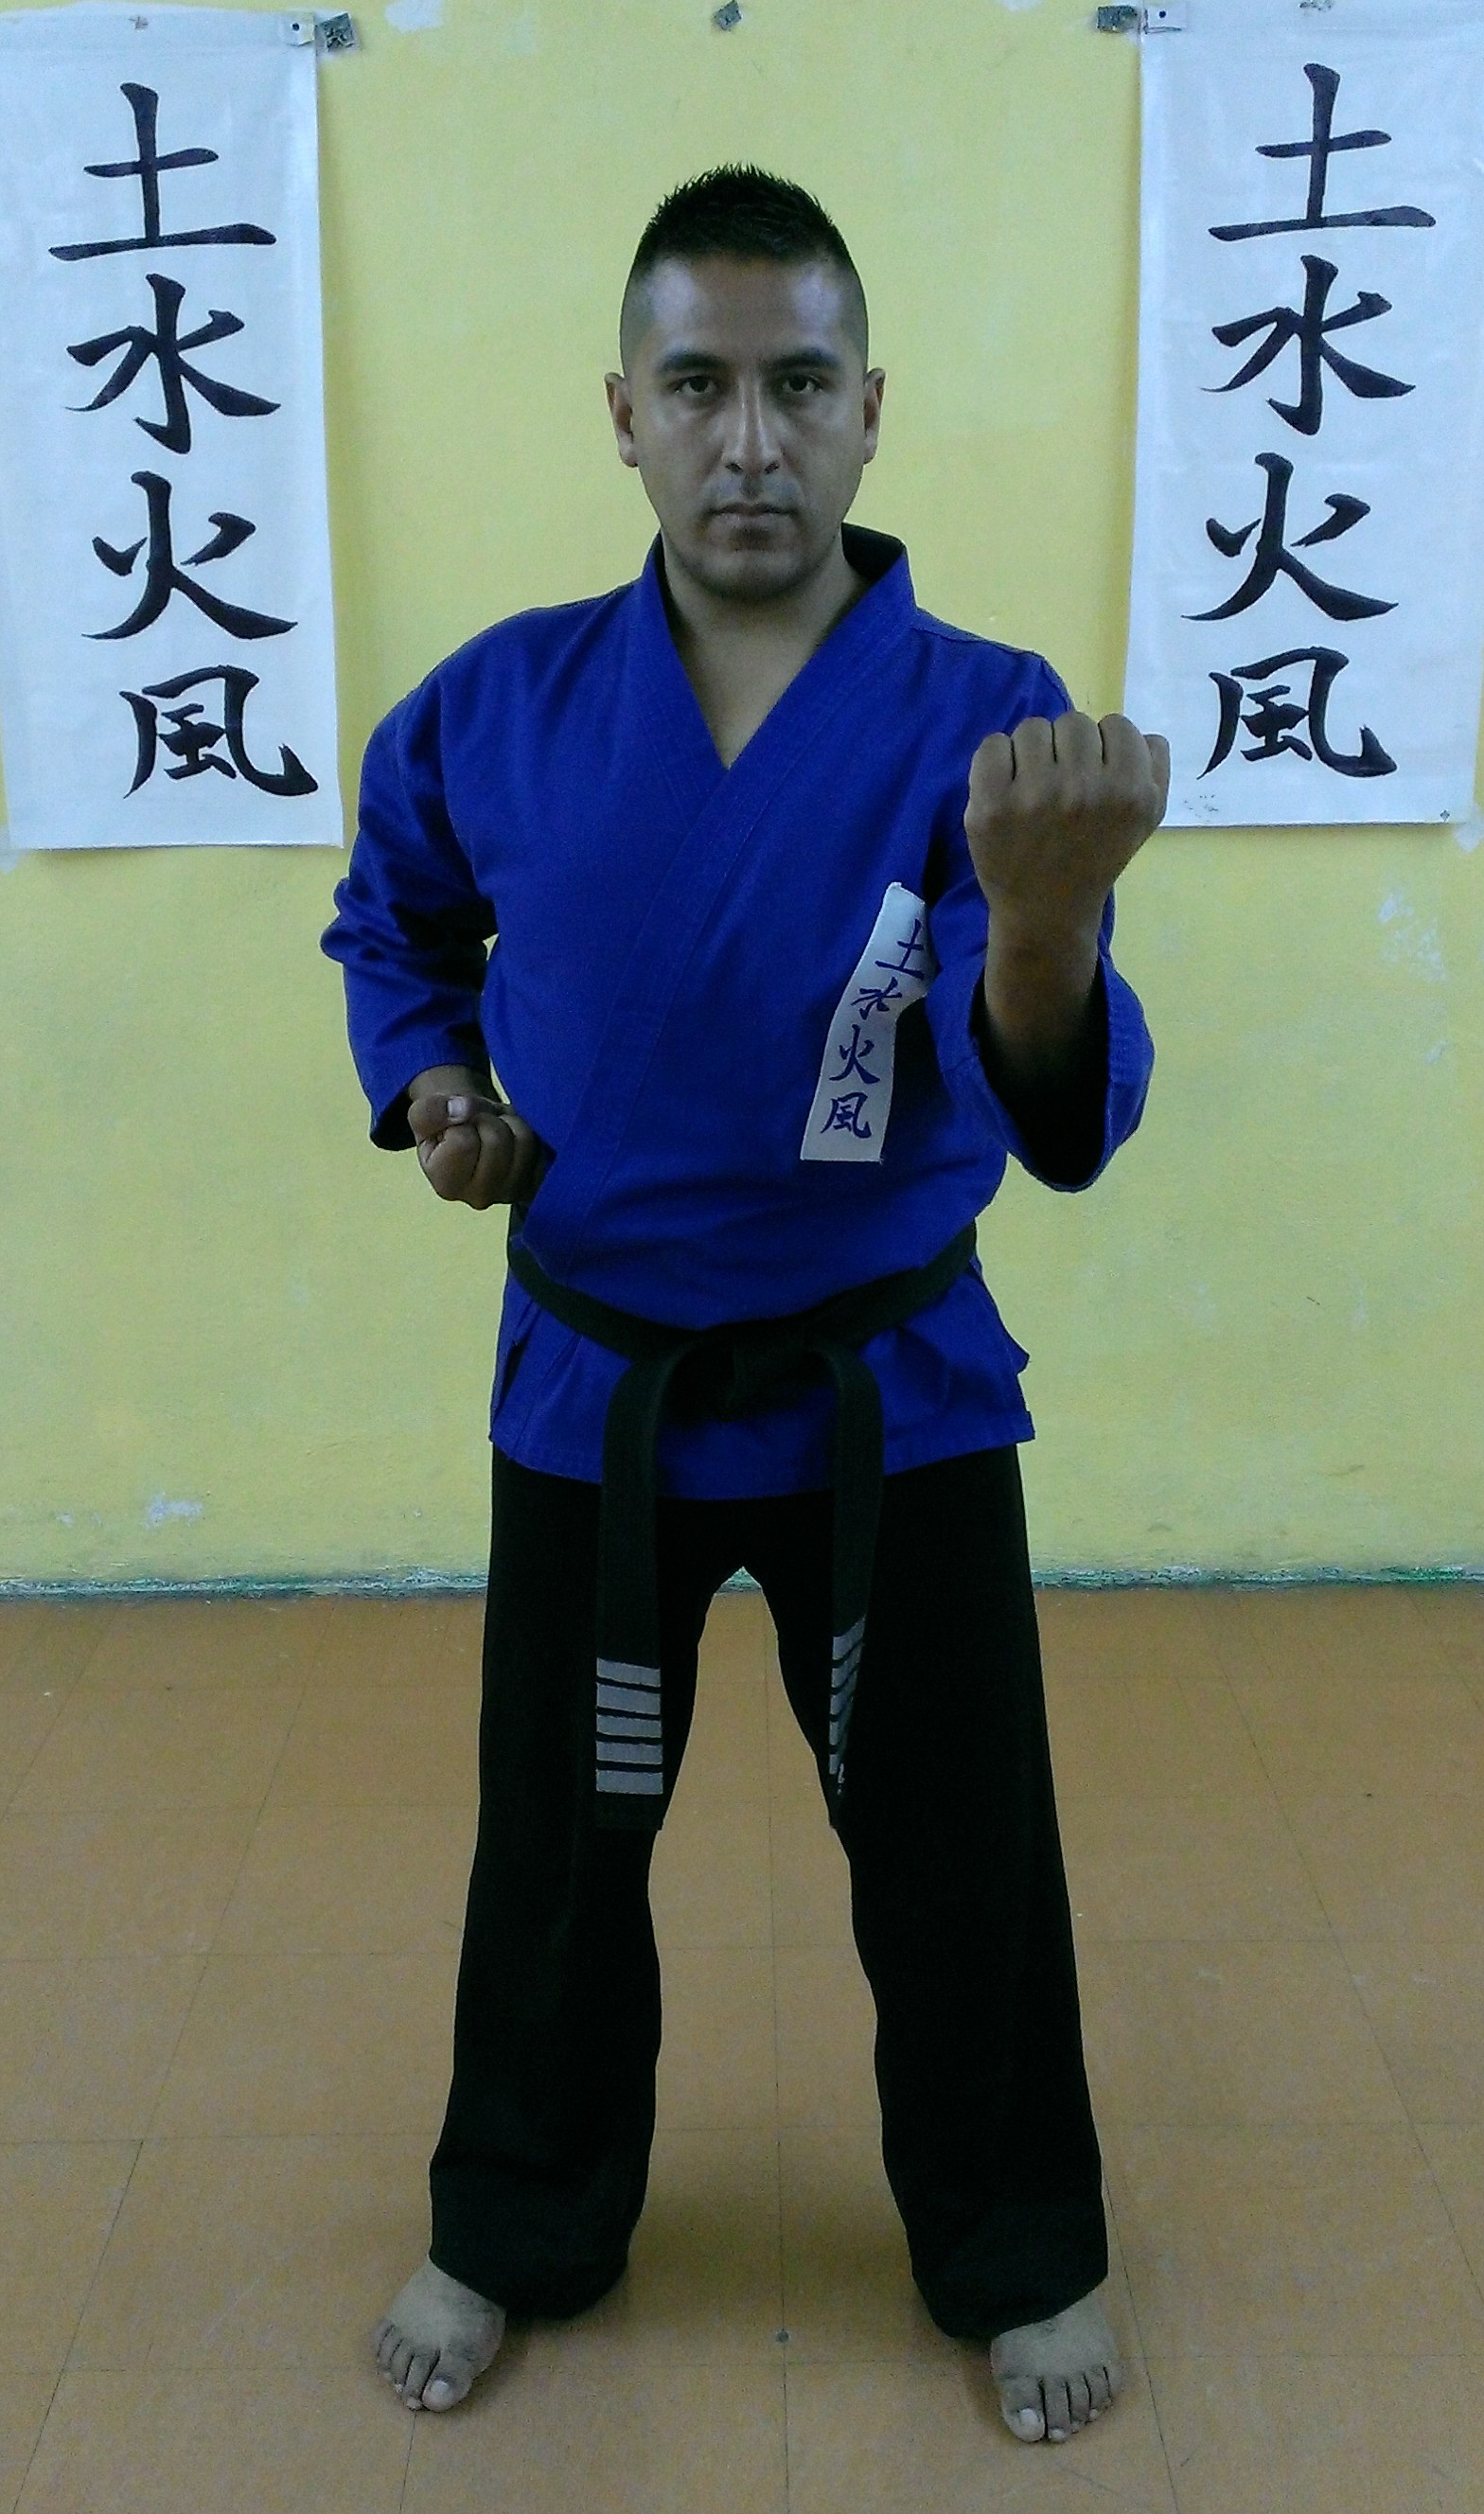
\includegraphics[width=5cm, height=8cm]{./Figuras/Tecnica/ShudanSotoUke_Frontal}}
	\subfloat[Defensa Shudan Soto Uke lateral]{
		\label{fig:ShudanSotoUke_Lateral}
		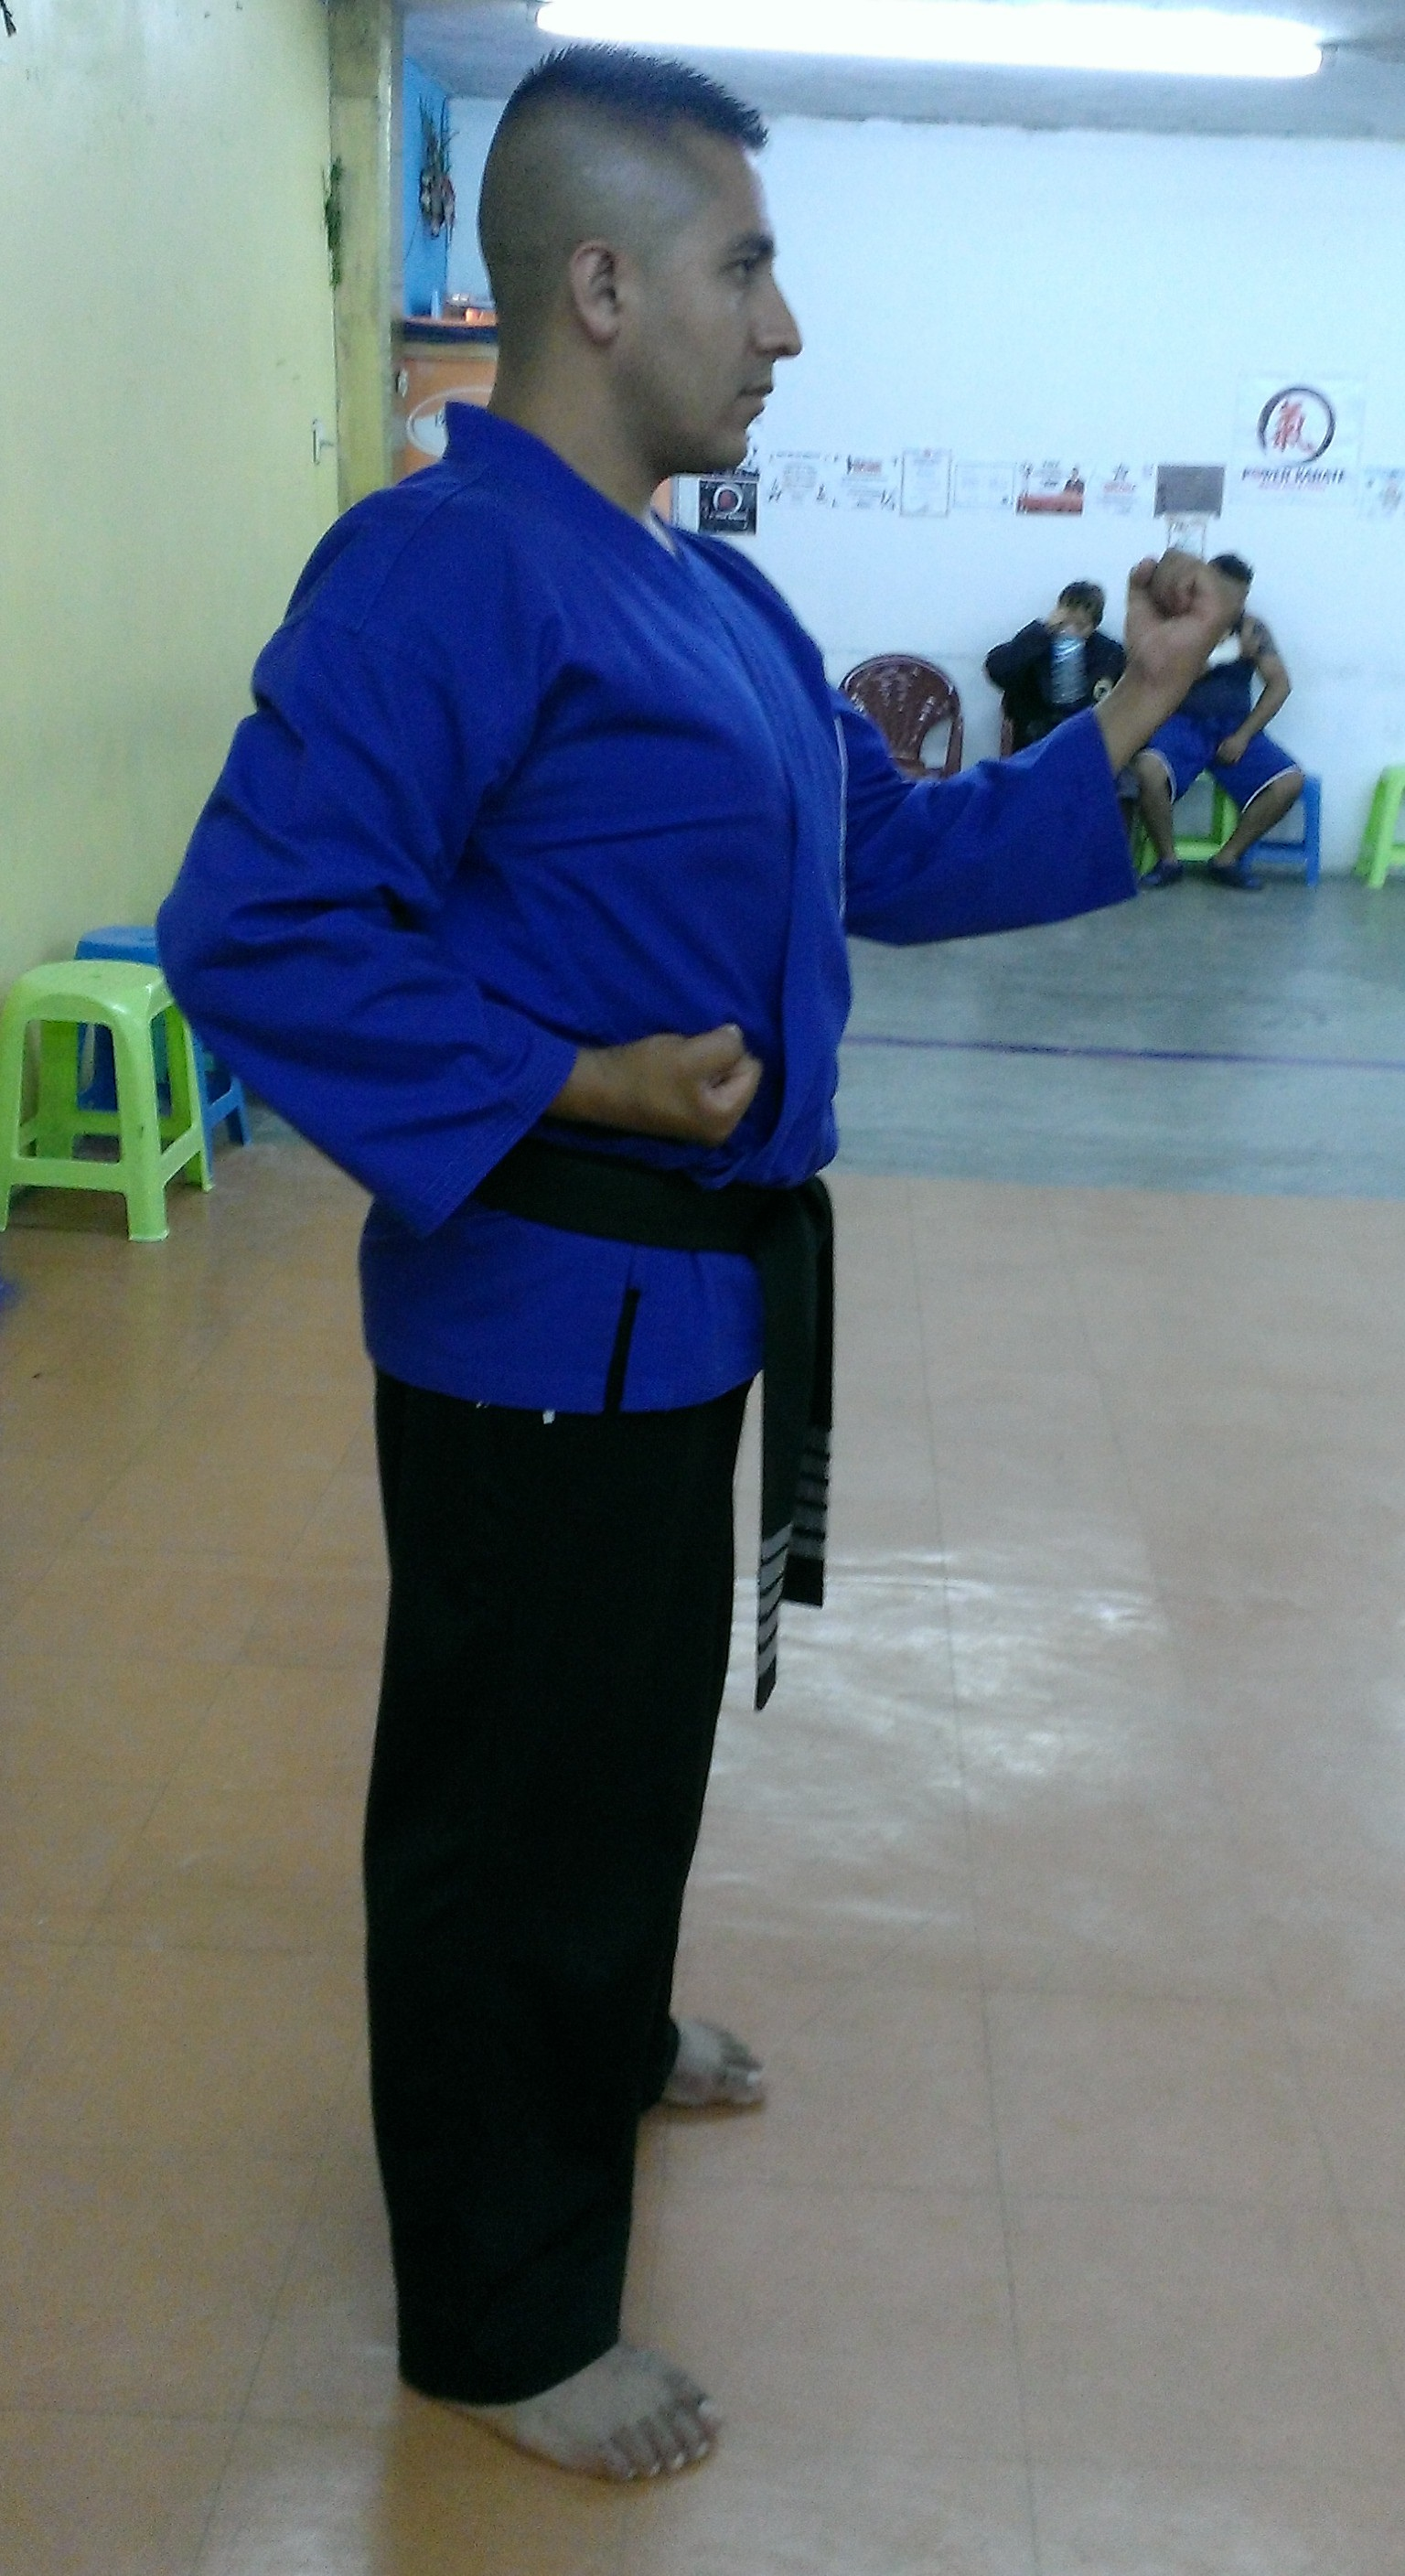
\includegraphics[width=5cm, height=8cm]{./Figuras/Tecnica/ShudanSotoUke_Lateral}}
	\caption{Defensa Shudan Soto Uke}
	\label{fig:Defensas2}
\end{figure}

\begin{figure}[H]
	\centering
	\subfloat[Defensa Yodan Age Uke frontal]{
		\label{fig:YodanAgeUke_Frontal}
		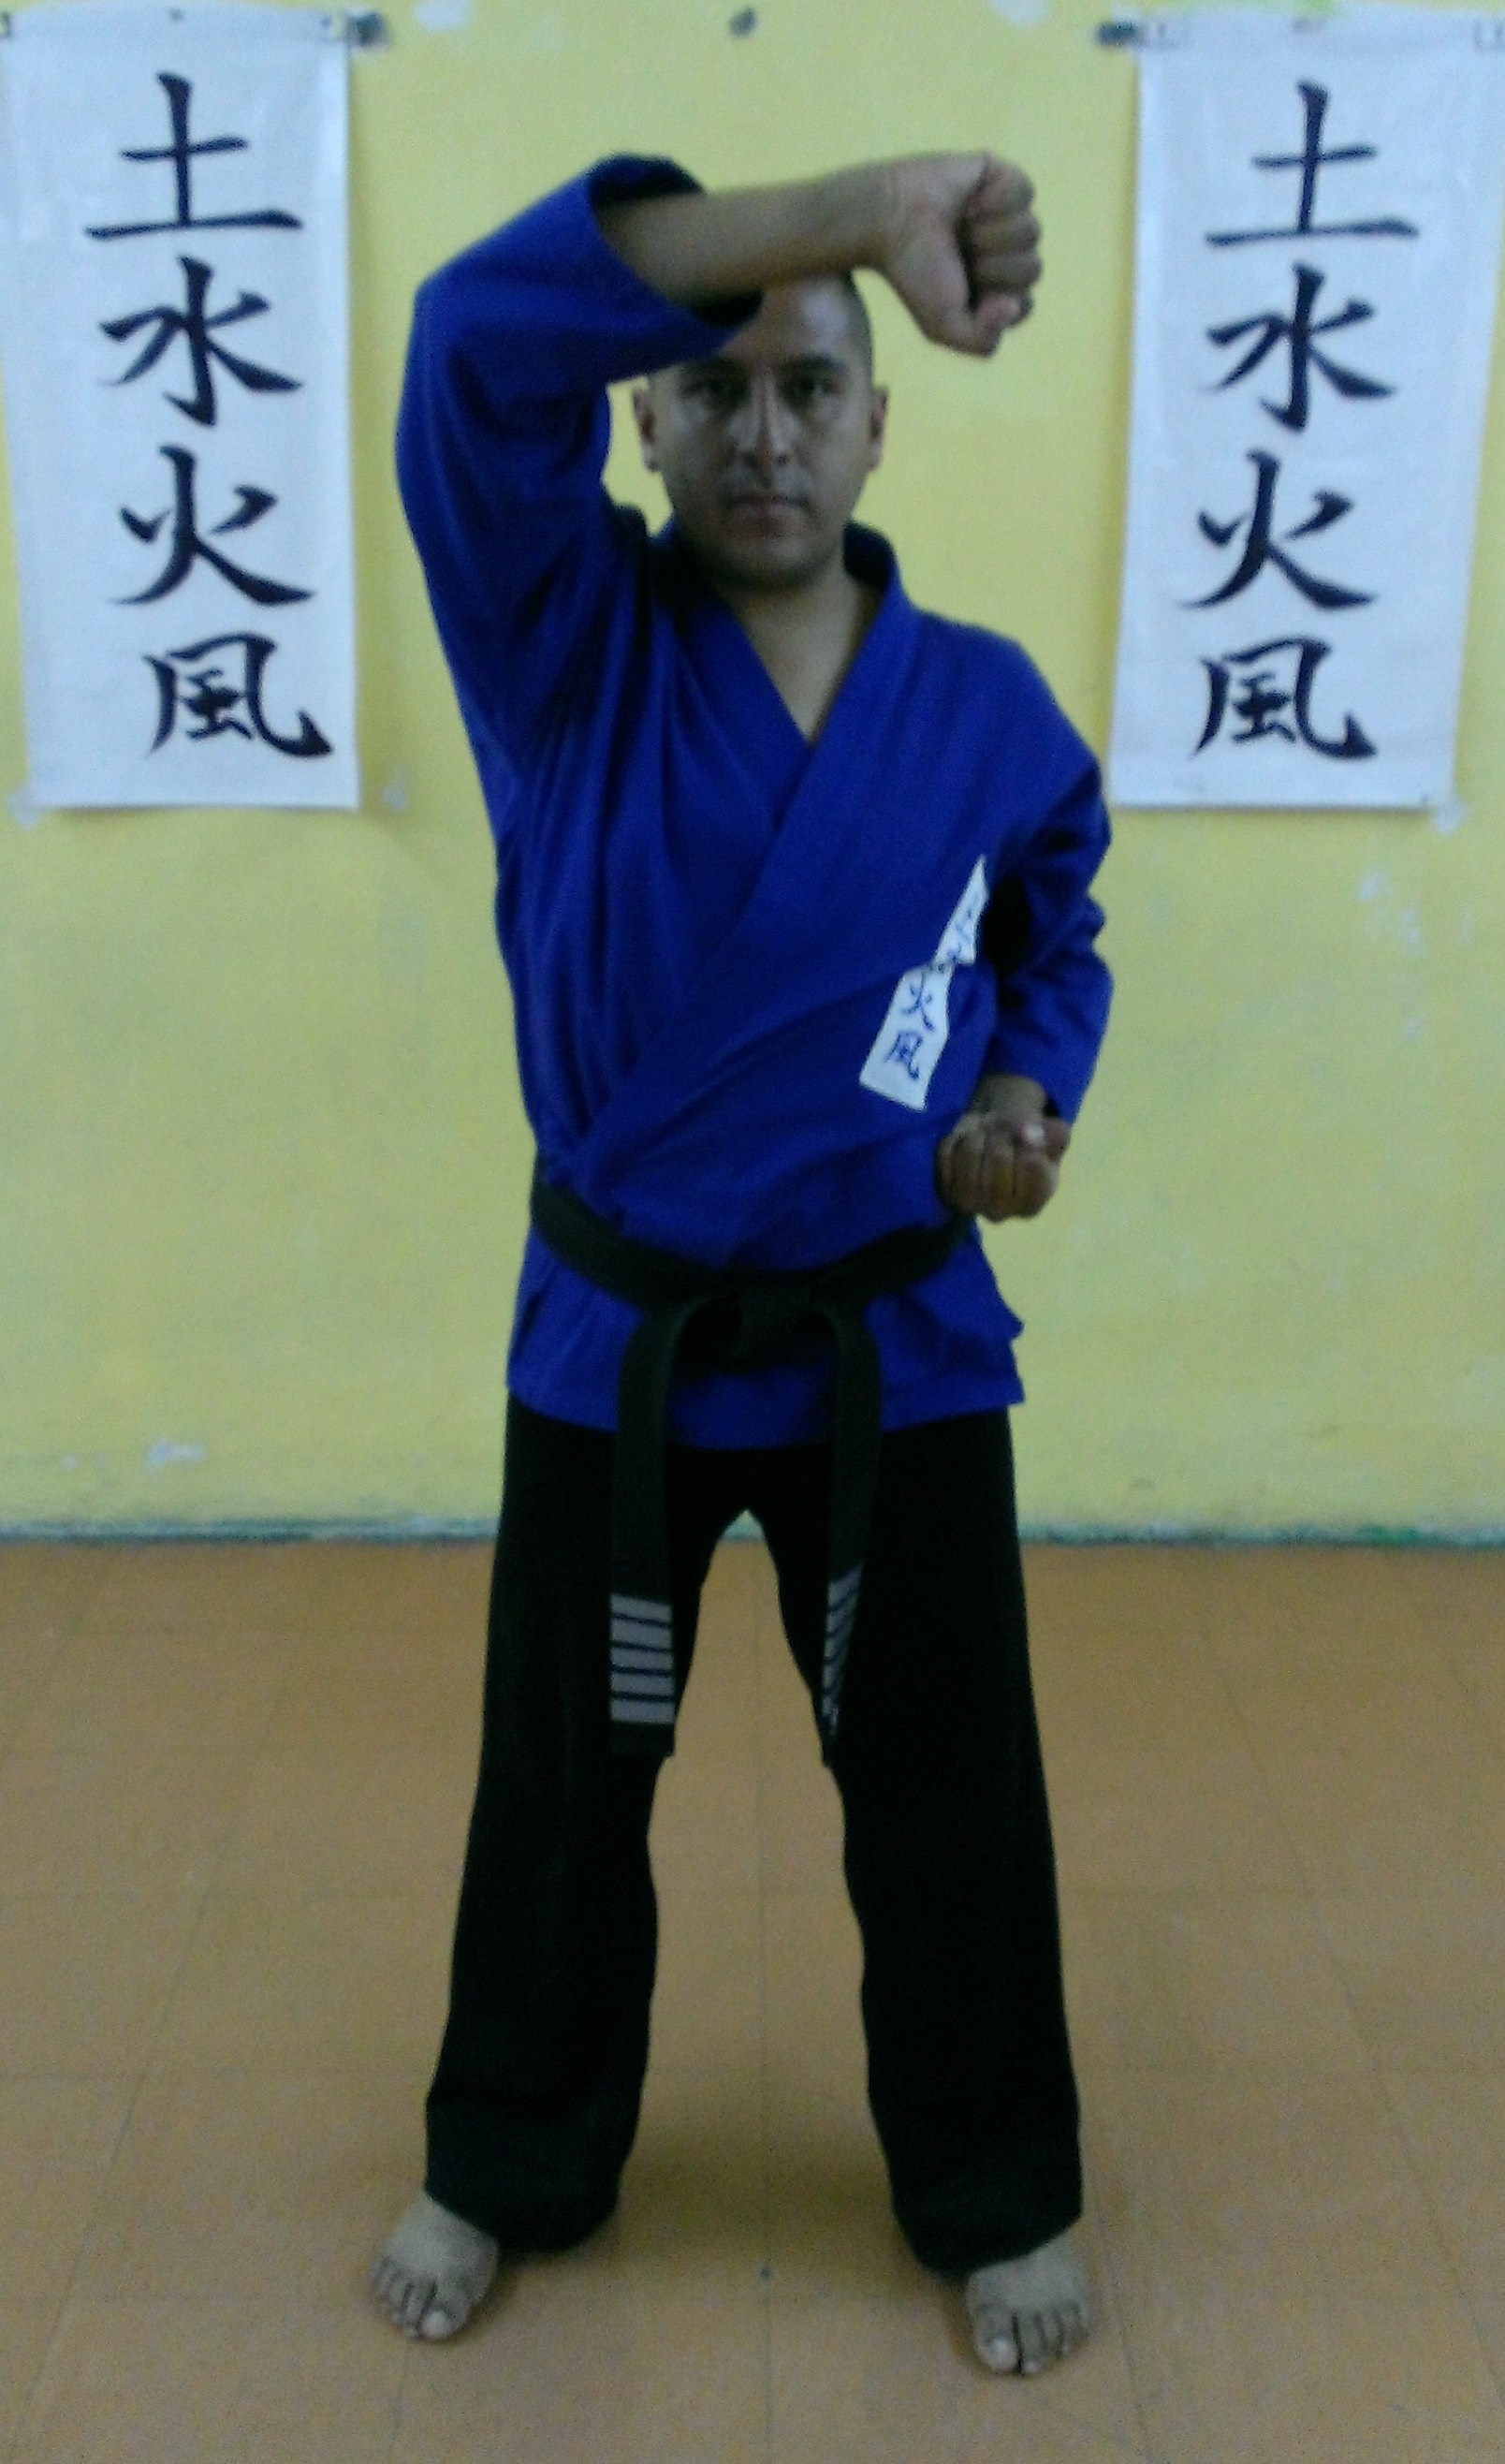
\includegraphics[width=5cm, height=8cm]{./Figuras/Tecnica/YodanAgeUke_Frontal}}
	\subfloat[Defensa Yodan Age Uke lateral]{
		\label{fig:YodanAgeUke_Lateral}
		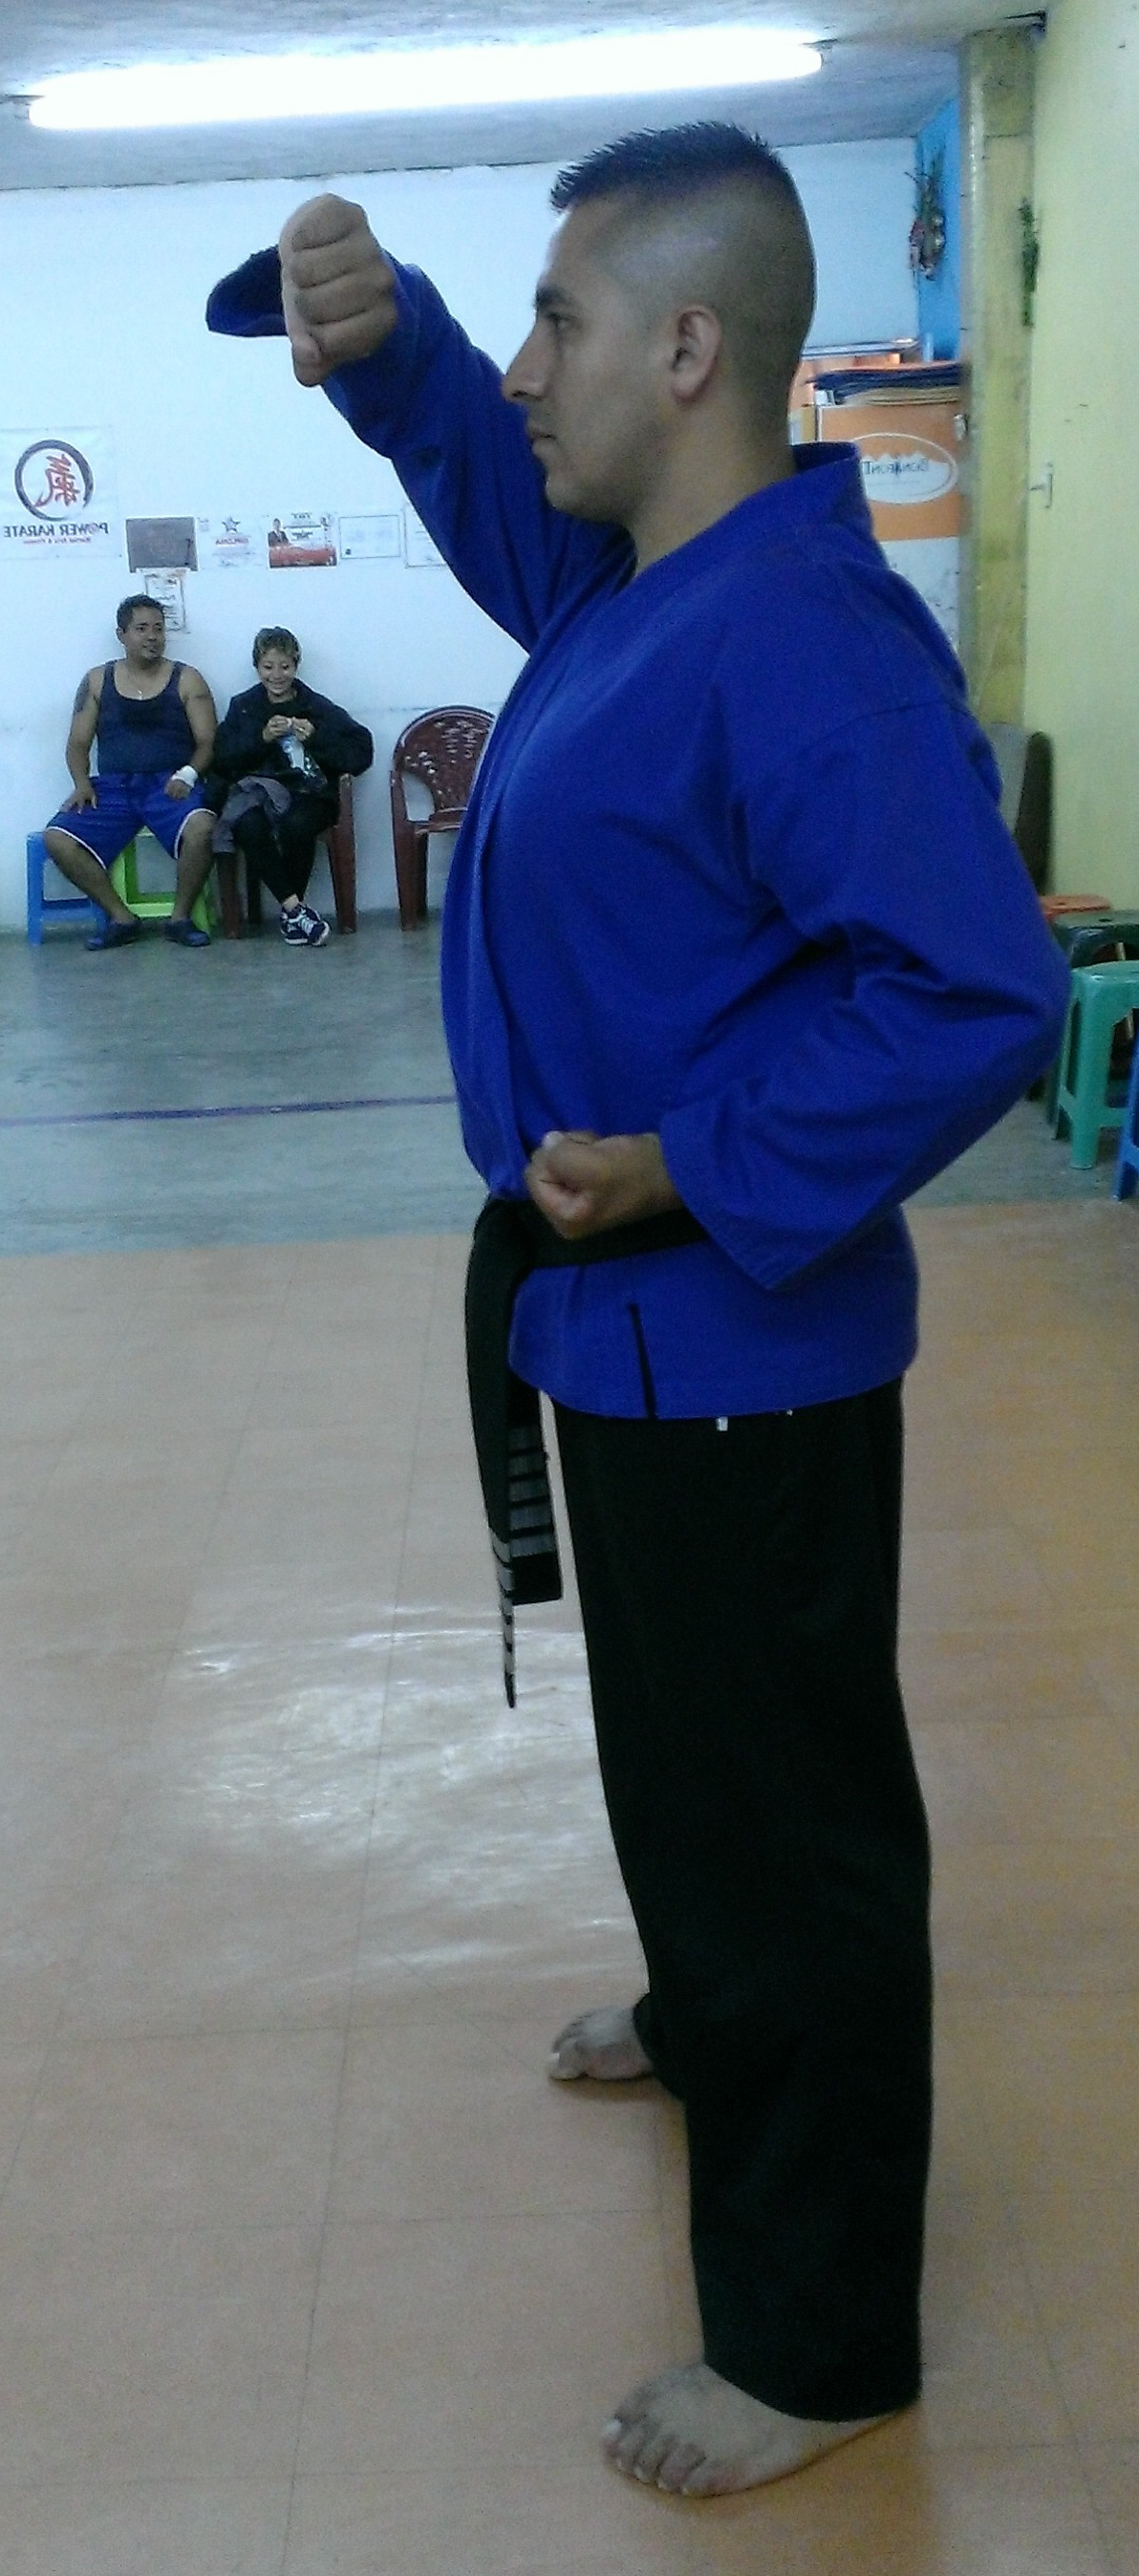
\includegraphics[width=4.5cm, height=8cm]{./Figuras/Tecnica/YodanAgeUke_Lateral}}
	\caption{Defensa Yodan Age Uke}
	\label{fig:Defensas3}
\end{figure}

\begin{figure}[H]
	\centering
	\subfloat[Ataque con brazo Seiken Tsuki frontal]{
		\label{fig:SeikenTsuki_Frontal}
		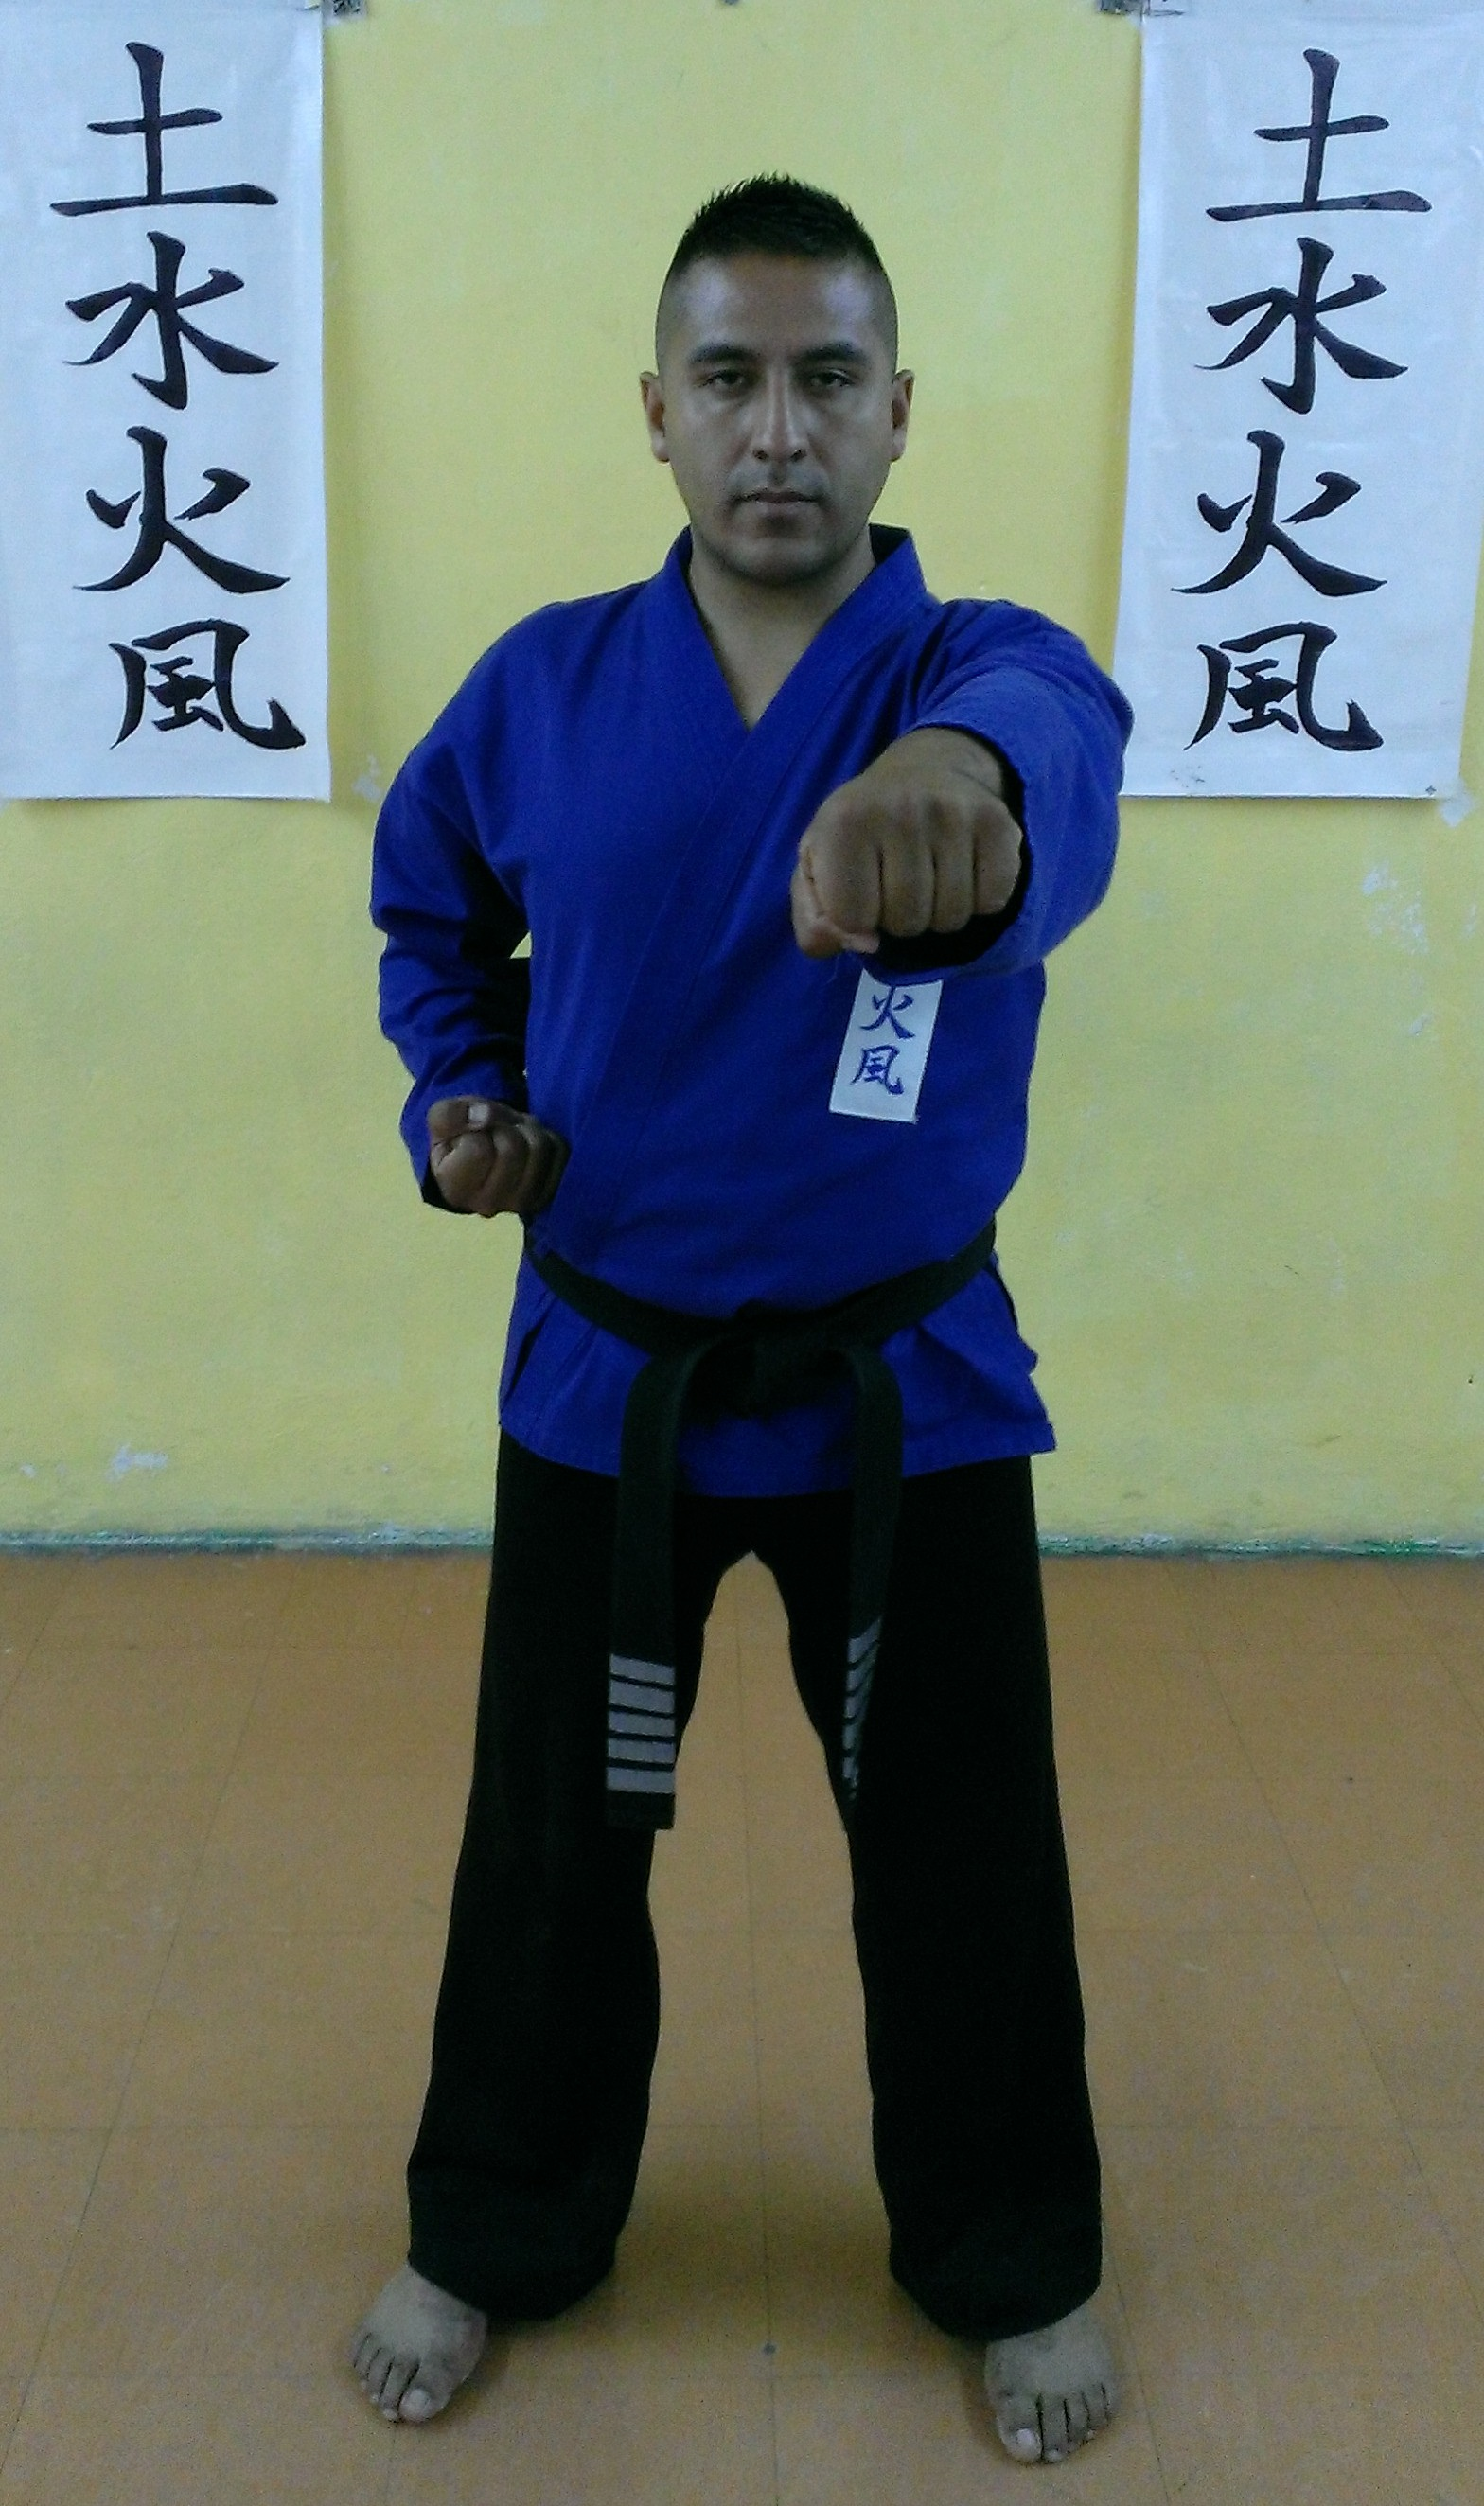
\includegraphics[width=5cm, height=8cm]{./Figuras/Tecnica/SeikenTsuki_Frontal}}
	\subfloat[Ataque con brazo Seiken Tsuki lateral]{
		\label{fig:SeikenTsuki_Lateral}
		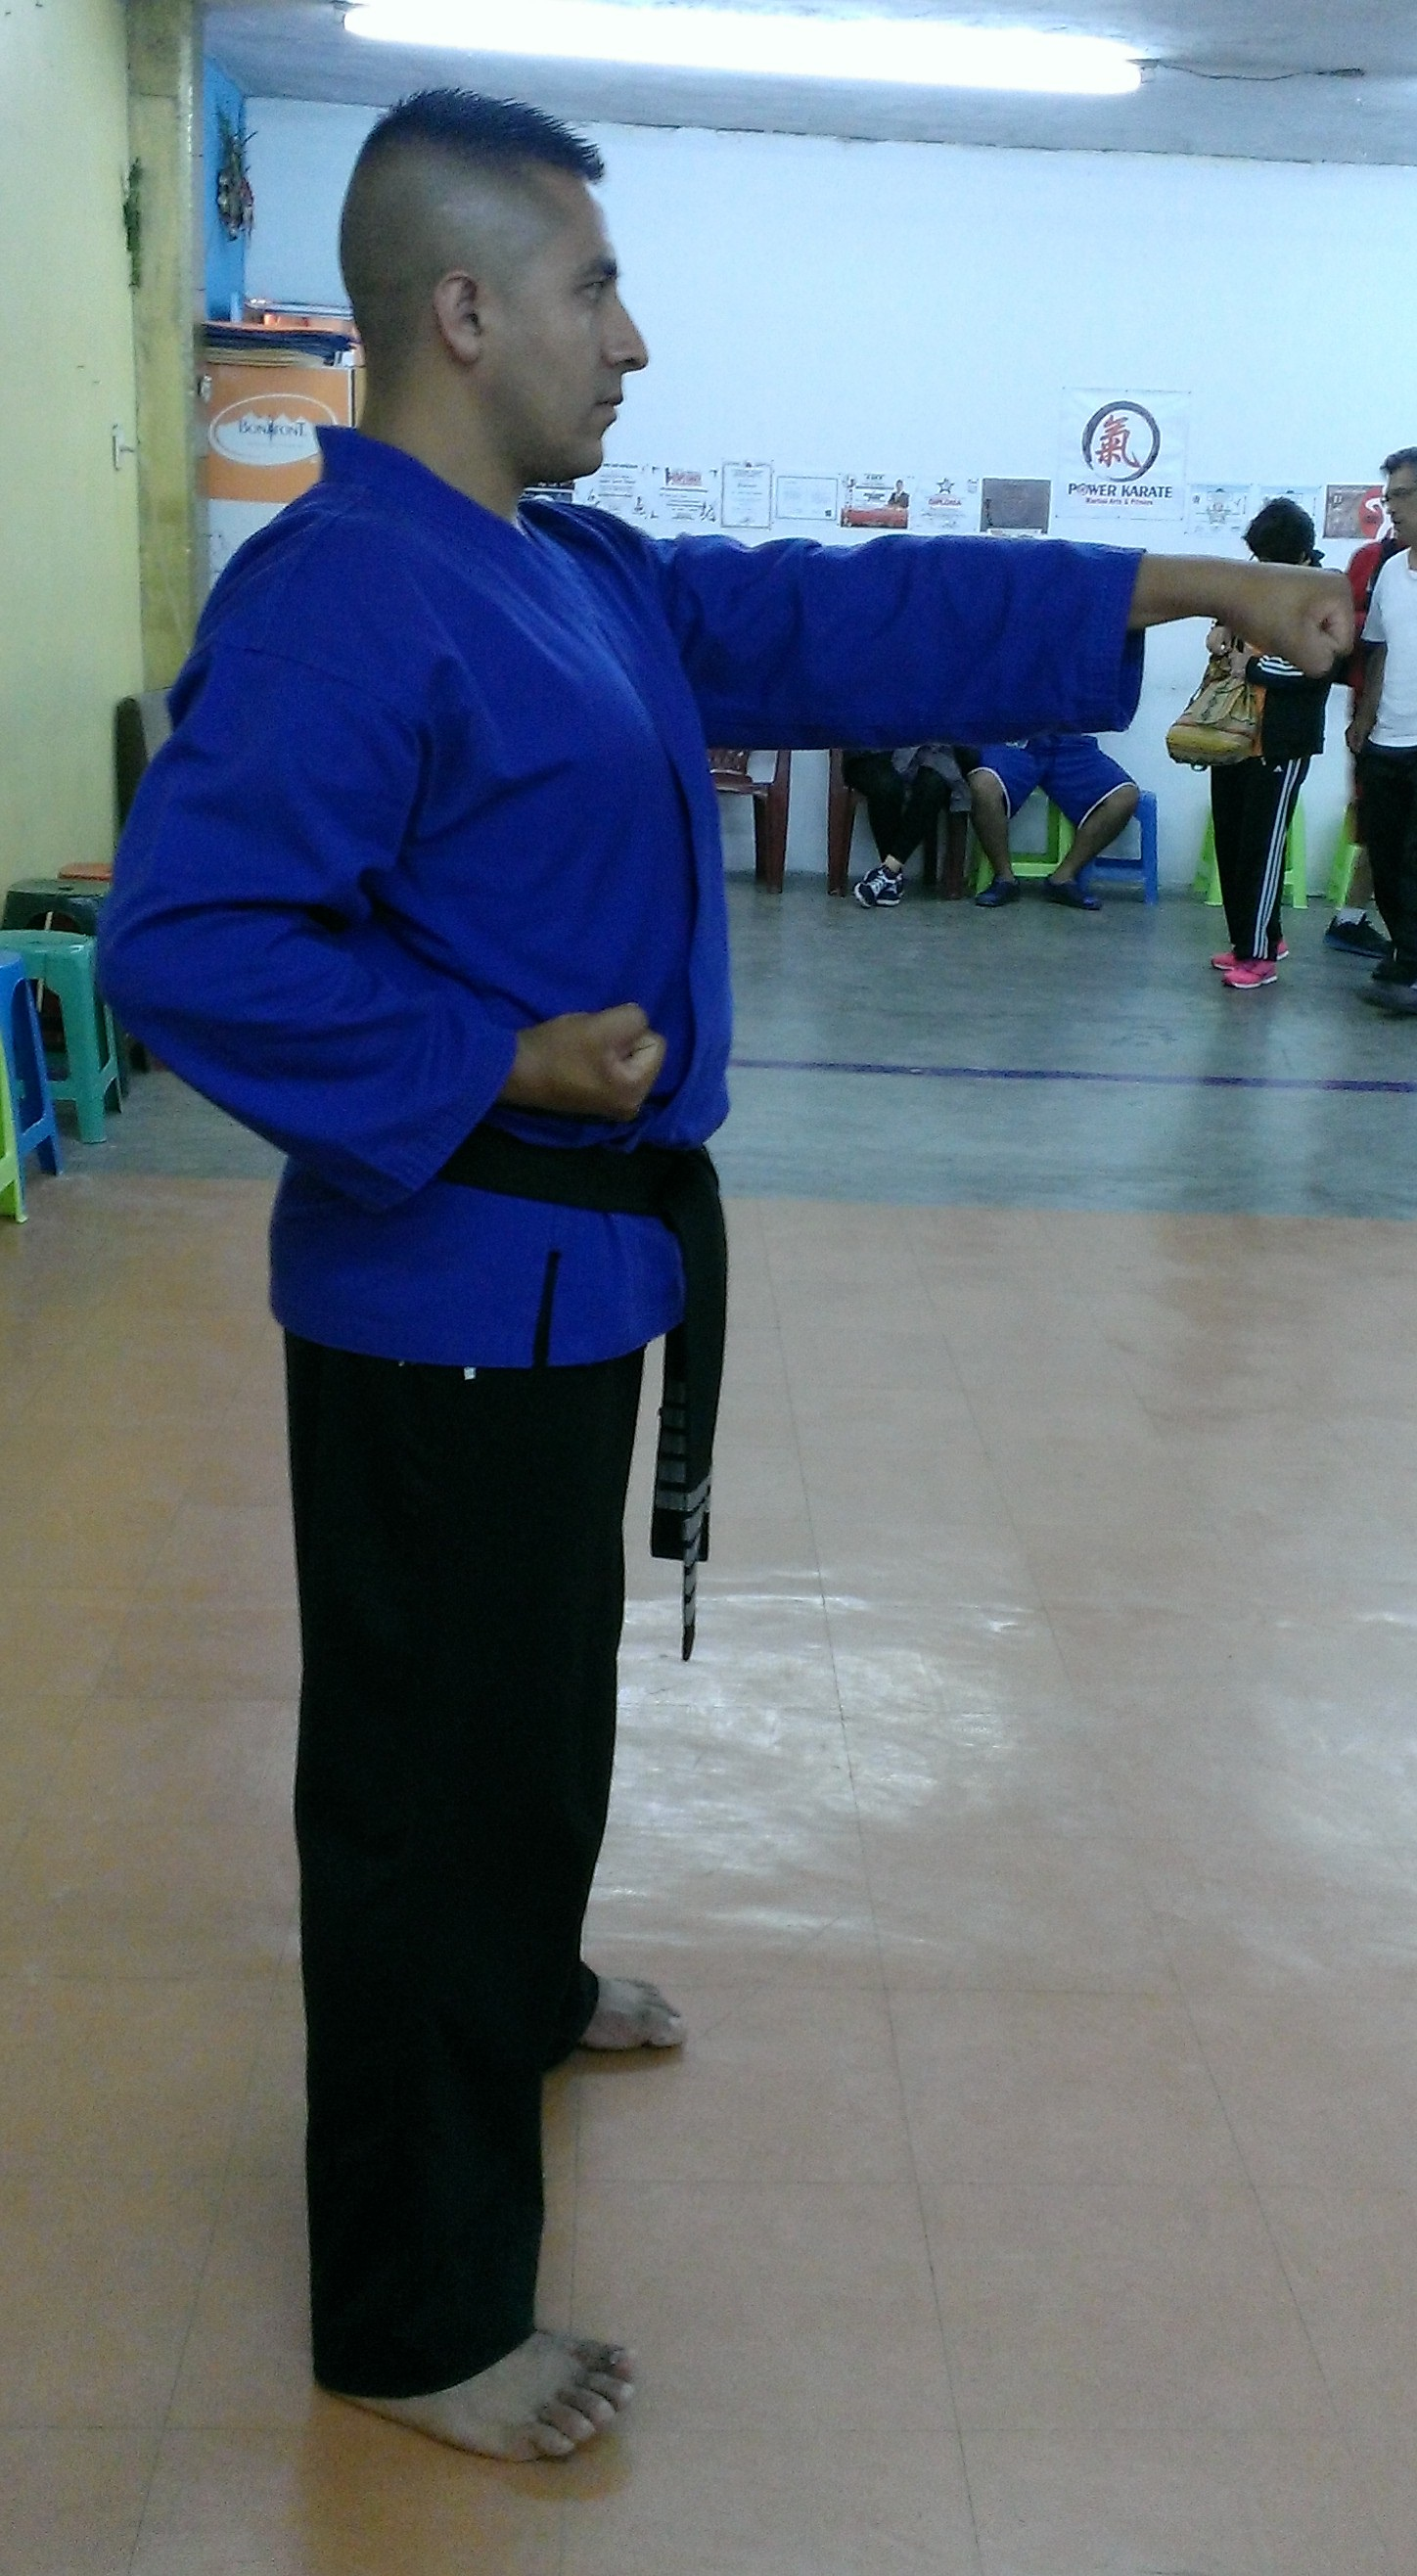
\includegraphics[width=5cm, height=8cm]{./Figuras/Tecnica/SeikenTsuki_Lateral}}
	\caption{Ataque con brazo Seiken Tsuki}
	\label{fig:Ataques1}
\end{figure}

\begin{figure}[H]
	\centering
	\subfloat[Ataque con pierna Mae Geri frontal]{
		\label{fig:MaeGeri_Frontal}
		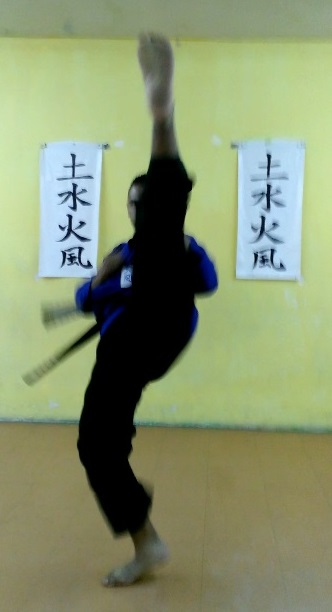
\includegraphics[width=5.5cm, height=8cm]{./Figuras/Tecnica/MaeGeri_Frontal}}
	\subfloat[Ataque con pierna Mae Geri lateral]{
		\label{fig:MaeGeri_Lateral}
		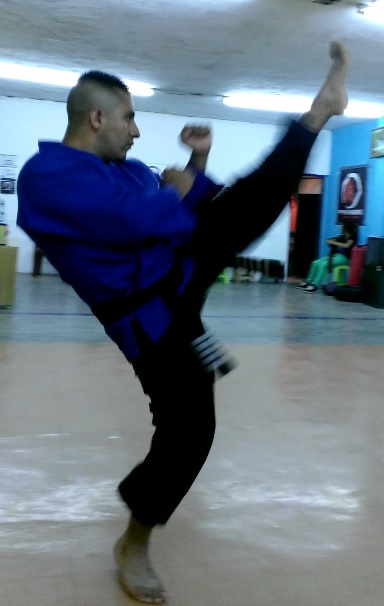
\includegraphics[width=5cm, height=8cm]{./Figuras/Tecnica/MaeGeri_Lateral}}
	\caption{Ataque con pierna Mae Geri}
	\label{fig:Ataques2}
\end{figure}

\clearpage
%-----------------------------------------------------------------------------
\subsubsection{Descripción de movimientos}
La siguiente tabla \ref{tab:DMT} \nameref{tab:DMT} muestra la descripción de los movimientos de técnica, clasificando el tipo de movimiento al que pertenece (posiciones, defensas o ataques).

\begin{table}[H]
\centering
\begin{tabular}{| p{4 cm} | p{2 cm} | p{9 cm} |}
\hline
\rowcolor[rgb]{0.529412, 0.807843, 0.980392} {\textbf{Nombre}} & {\textbf{Tipo}} & {\textbf{Descripción}}\\
\hline
\textbf{Musubi - dachi} &  Posición. & Talones juntos, puntas de los pies separadas, manos a los costados.\\
\hline
\textbf{Hachiji - dachi} &  Posición. & Piernas separadas a la altura de los hombros, puntas de los pies hacia el frente, brazos estirados hacia el frente.\\
\hline
\textbf{Senkuntsu - dachi} &  Posición. & Una pierna flexionando la rodilla y la otra pierna estirada hacia atrás, teniendo una separación entre ellas.\\
\hline
\textbf{Gedan Barai Uke} &  Defensa. & Brazos con los puños cerrados, uno en la cintura y el otro estirado hacia abajo con una separación sobre el cuerpo.\\
\hline
\textbf{Shudan Soto Uke} &  Defensa. & Brazos con los puños cerrados, uno en la cintura y el otro realizando una flexión del codo poniendo el puño a la altura del hombro separados por un espacio entre ellos.\\
\hline
\textbf{Yodan Age Uke} &  Defensa. & Brazos con los puños cerrados, uno en la cintura y el otro realizando una flexión del codo, poniendo el antebrazo a una altura ligeramente mayor a la cabeza.\\
\hline
\textbf{Seiken Tsuki} &  Ataque. & Brazos con los puños cerrados, uno en la cintura y el otro realiza un golpe hacia el frente, a la altura de su pecho.\\
\hline
\textbf{Mae Geri} &  Ataque. & Una pierna apoyada en el sueño y la otra realiza una patada hacia el frente a la altura de su estómago, pecho o cabeza.\\
\hline
\end{tabular}
\caption{Descripción de movimientos de técnica}
\label{tab:DMT}
\end{table} 
%------------------------------------------------------------------------------------
\section{E-Learning}

Con la población en Internet, la demanda de e-Learning ha incrementado recientemente \cite{Chang}. E-Learning representa una aproximación casi ideal para el desarrollo flexible y rentable de competencias desde que pueden ser usadas sin restricciones relacionadas con las ubicaciones físicas y el tiempo de uso \cite{Cukusic}. Una de las principales características del e-Learning es la capacidad de integrar diferentes medios, como texto, imágenes, audio, animaciones y video para crear instrucciones multimedia, promoviendo los intereses de lectura y disposición del aprendiz \cite{Vichuda}. De manera que, la investigación ha mostrado que el diseño de recursos multimedia es costoso y no tienen efectos consistentes en promover el desarrollo del aprendizaje. Por ejemplo, el material didáctico multimedia es menos importante que el proceso y la función del sistema, con el fin de producir un efecto significativo en la comprensión del contenido educativo, aunque de esta forma llame más la atención del aprendiz \cite{Bartscha}. Además, algunas investigaciones muestran que demasiados elementos multimedia innecesarios pueden distraer a los aprendices \cite{Clark}. También, el diseño y desarrollo de recursos multimedia didacticas es costoso, aunque el rapido progreso de las tecnologías de la computación e Internet hacen tal esfuerzo posible \cite{Sun}. No obstante los elementos multimedia son muy importantes para el usuario o aprendiz para utilizar una sistema basado en e-Learning. Por lo tanto, la forma de desarrollar y apoyar los contenidos multimedia efectivos de aprendizaje basadas en el mejor ajuste del alumno de acuerdo con el curso de aprendizaje se está convirtiendo en un problema importante de e-Learning. Con respecto a la evaluación de la evidencia científica, que distribuyen e identifican la calidad del sistema de enseñanza. \\

La educación tradicional en salones de clase no siempre satisface todas las necesidades del nuevo mundo para que el aprendizaje sea permanente. El e-Learning, hace referencia al aprendizaje vía Internet, provee a las personas una forma flexible y personalizada de aprender. Ofrece oportunidades de aprendizaje en demanda y reduce los costos \cite{Zhang}. \\

Enseñar y aprender ya no son exclusivos dentro de un salón de clases tradicional \cite{NC}. Los métodos de aprendizaje necesitan ser más portables y flexibles. El nuevo enfoque del aprendizaje a distancia es construir una infraestructura de costo efectivo que permita el aprendizaje en cualquier tiempo, en cualquier lugar, autodidacta y de forma interactiva.\\

El aprendizaje tradicional cara-a-cara tiene sus ventajas de ser familiar, cercano y confortable tanto para instructores como para estudiantes. Sin embargo, puede requerir viajar e interrumpir el trabajo, causando una pérdida de tiempo. En algunas situaciones, enviar al instructor al lugar puede ser impráctico. El e-Learning sirve como un mecanismo complementario para el aprendizaje remoto o permanente \cite{Zhang}.
%------------------------------------------------------------------------------------
\subsection{E-Learning asíncrono}
\label{sec:elearning}
El e-Learning asíncrono no requiere la participación simultánea de los aprendices e instructores. Se refiere a una situación de aprendizaje donde el evento de aprendizaje no toma lugar en tiempo real \cite{Zhang}. Las personas pueden aprender en cualquier tiempo. Por lo tanto, el e-Learning asíncrono es aprendizaje bajo demanda, lo cual les da a los aprendices más control sobre el proceso del aprendizaje y el contenido.\\

Por las características de este tipo de aprendizaje, se opta por tomar su concepto para ser utilizado en el presente trabajo terminal.
%------------------------------------------------------------------------------------
\subsection{Beneficios del E-Learning}

\begin{itemize}
\item Ahorros de costo y tiempo: Hasta un 40\% del dinero gastado en el aprendizaje individual, es abarcado por el costo del viaje \cite{Zhang}. Desde que los e-Learners no tienen que viajar hasta una locación específica, el e-Learning puede permitir un ahorro en los costos o en gastos indirectos.
\item Aprendizaje autodidacta: El e-Learning fomenta el aprendizaje autodidacta y autodirigido estructurando actividades centradas en el aprendiz. Cada aprendiz puede seleccionar las actividades de aprendizaje  que mejor se adecue a su entorno, intereses y su carrera en ese momento.
\item Ambiente de aprendizaje colaborativo: El e-Learning une a los aprendices y expertos separados físicamente para formar un aprendizaje colaborativo en línea \cite{Hiltz}.
\item Mejor acceso a los instructores: En un ambiente de e-Learning, los aprendices obtienen de los instructores ayuda y orientación en línea.
\end{itemize}

\clearpage
\section{Algoritmo Dynamic Time Warping}
\label{sec:DTW}

Dynamic time warping, es una técnica que encuentra la alineación óptima entre dos series de tiempo, es un algoritmo para medir la similaridad entre dos secuencias, las cuales pueden variar en el tiempo o la velocidad.\\
Puede ser utilizado para encontrar regiones correspondientes entre las dos series o para determinar la similitud entre las dos series de tiempo.\\

Se utiliza a menudo en el reconocimiento de voz para determinar si dos formas de onda representan la misma frase hablada. En una forma de onda del habla, la duración de cada sonido hablado y el intervalo entre sonidos pueden variar, pero las formas de onda del habla deben ser similares.\\
También se ha encontrado útil en muchas otras disciplinas, incluyendo la minería de datos, reconocimiento de gestos, la robótica y la medicina \cite{DTW}.

La distancia euclidiana entre dos series de tiempo no es más que la suma de las distancias cuadradas de cada punto enésimo en una serie de tiempo hasta el punto enésimo en la otra.\\
El principal inconveniente de la utilización de la distancia euclidiana para datos de series de tiempo es que: si dos series de tiempo son idénticas, pero una se desplaza ligeramente a lo largo del eje de tiempo, entonces la distancia euclídea puede considerar que son muy diferentes la una de la otra.\\
DTW se introdujo para superar esta limitación, haciendo caso omiso de los cambios globales y locales en la dimensión de tiempo.\\

En general, el funcionamiento del algoritmo se basa en la búsqueda de un camino óptimo de coincidencia entre dos secuencias con ciertas restricciones. Las secuencias son transformadas no linealmente en el tiempo, de modo que son comprimidas o expandidas en el tiempo para que tengan el mismo largo, y así poder compararlas punto a punto. \\

\textbf{Algoritmo de alineamiento temporal dinámico:} \\

Supongamos que queremos comparar y evaluar la diferencia entre dos señales, supongamos que tenemos dos series de tiempo, un secuencia Q de longitud n, y una secuencia C de longitud m, donde: \\
Q = q1, q2, ..., qi, ..., qn 	(1)\\
C = c1, c2, ..., cj, ... cm 	(2)\\

Para alinear estas dos secuencias utilizando DTW, primero construimos una matriz de n por m,  $d(q_i,c_j) = d(q_i - c_j)^2$, que es la alineación entre los puntos  $q_i$ y $c_j$.\\
Para encontrar la mejor coincidencia entre estas dos secuencias, recuperamos un camino a través de la matriz que minimiza la distancia total acumulada entre ellos, como se ilustra en la Figura. En particular, la ruta óptima es el camino que minimiza el coste.\\

$DTW(Q,C)=min\left\{{\sqrt[]{\sum_{k=1}^K{w_k}}}\right\}$ \\

donde $w_k$ es el elemento de matriz $(i, j)_k$ que también pertenece al k-ésimo elemento de un camino de deformación $W$, un conjunto contiguo de elementos de la matriz que representan un mapeo entre $Q$ y $C$.\\

Este camino se puede encontrar utilizando programación dinámica para evaluar la siguiente repetición.\\
$ \gamma (i, j) = d (q_i, c_j) + min \left\{{\gamma (i-1, j-1), \gamma (i-1, j), \gamma (i, j-1)}\right\} $ \\

donde $d(i, j)$ es la distancia que se encuentra en la celda actual, y $\gamma (i, j)$ es la distancia acumulada de $d (i, j)$ y las distancias acumulativas mínimos de las tres células adyacentes.\\

\begin{figure}[h]%La h significa que la colocara cerca del texto
	\begin{center}
		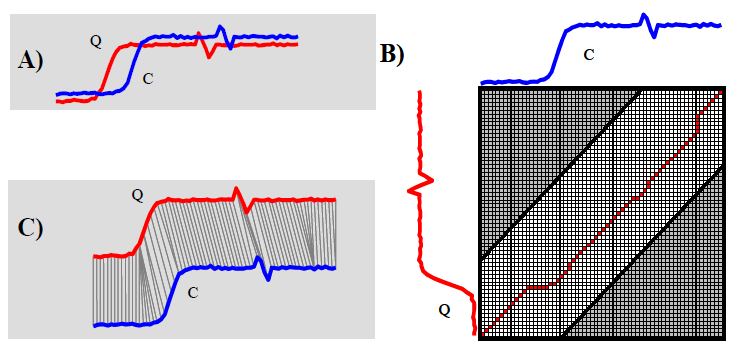
\includegraphics[scale=0.55]{./Figuras/DTWGraficas}
	\end{center}
	\caption{Comparación de dos señales de tiempo con DTW}
	\label{fig:comparacionsenalesdtw}
\end{figure}

La Figura (A) muestra dos secuencias similares Q y C, pero fuera de fase.\\
La Figura (B) para alinear las secuencias, se construye una matriz de deformación y la búsqueda de la ruta óptima, que se muestra con los cuadrados sólidos.\\
La Figura (C) muestra la alineación resultante.\\

Esta secuencia debe satisfacer tres condiciones:\\

1.-Condición de frontera: $p_l=(1,1)$ y $p_L=(N,M)$\\
   Para que los primeros  y los últimos elementos de X e Y estén alineados y así las secuencias completas estén alineadas.\\
   
2.-Condición de monotonía:  $n_1<= n_2<=...n_L $ y $ m_1 <= m_2 <= ... m_L$ \\
   Nos aseguramos de que elementos que se sucedan en el tiempo también se sucedan al ser alineados.\\
   
3.-Condición de salto: Nos indica que no se puede omitir ningún elemento de X e Y y que el camino de alineamiento es continuo.\\

Para reducir el número de rutas a considerar durante el cómputo, varias limitaciones conocidas (condiciones de frontera, la condición de continuidad, condición monótona y Ajuste Ventana Estado) se han aplicado al problema de restringir los movimientos que se pueden hacer desde cualquier punto la ruta de acceso y así restringir el número de caminos que necesitan ser considerados.\\

\clearpage

